\clearpage
\phantomsection\addcontentsline{toc}{section}{报告 III --- Lefschetz 公式}
\begin{center}
{\Large \textbf{SGA 5 --- 报告 III}}\\[0.4em]
{\large \textbf{Lefschetz 公式}}\\[0.3em]
A.~Grothendieck 著，L.~Illusie 整理
\end{center}

本报告按照 Verdier 的表述（参见~[18]），证明平展上同调中层复形之间对应的 Lefschetz 公式。约十年前由 IHES 散发的早期版本在解消假设下陈述了该公式，但未证明所需的相容性。Deligne 的有限性定理（SGA~$4^{1/2}$，有限性）使我们能够去掉这些假设，只需在域上分离有限型概形的范围内工作。至于相容性，整理者已经（颇费力地）逐一验证。

首先说明，这里的 Lefschetz 公式与它所推广的常系数迹公式（SGA~$4^{1/2}$，圈）一样，本质上是平凡的：它只是将对偶形式体系中的某些相容性写成公式。粗略地说，它断言，在一定条件下，超上同调复形 $R\Gamma(X,L)$（其中 $L$ 是 $X$ 上的层复形）的一个自同态的迹，可以算作 $X\times X$ 上某些上同调类的“积分”。实际考虑的自同态通常与对应 $C\subset X\times X$ 相联系，而在乘积上得到的类的支集包含于 $C\cap\Delta$，其中 $\Delta$ 是对角线；这些类在不动点的一个邻域内具有“局部性质”，原则上有利于计算。准确陈述见 4.2 和 4.7。事实上，若不把这些“局部”类用较易理解的不变量算出，当前公式便不会有什么意义；而迄今仅在很特殊的情形中进行了这样的计算（见 4.10、4.11 及下一报告，后者尤其处理曲线上 Frobenius 对应的情形）。

由于尚无合适的 $\ell$ 进层导出范畴（遗憾的是 Jouanolou 的学位论文未能发表），我们始终采用挠系数（其阶与剩余特征互素）。尽管定义迹时有一些小的技术困难，这一观点实际上给出更精细的公式；当计算局部项时希望通过覆盖使有关层平凡化，这些公式也更便于使用（尤其见（SGA~$4^{1/2}$，报告）、III~B 和 XII）。

第~1 节固定记号，并回顾（SGA~$4^{1/2}$，有限性）中在下文起关键作用的各种 Künneth 公式。我们还引入若干纤维范畴和余纤维范畴，借此简化后续某些相容性的验证。第~2 节技术性很强，初读时可略过。其主要结果（2.5）表达 $\RHom$ 的外张量积、正像与基变换之间的相容性。第~3 节定义复形之间的上同调对应，并说明它们如何作用于超上同调；上述结果使这一作用有几种等价描述。报告的核心是第~4 节：为便于以后计算局部项，我们在比通常情形显著更一般的相对情形中定义上同调对应的 Verdier 配对，并证明 Lefschetz 公式，同时给出常系数对应的最直接推论。第~5 节简要说明如何将常系数对应的某些通常构造（参见~[12]），例如取对偶、复合和外张量积，推广到复形之间的对应。大部分验证与前几节类似，故予以省略。最后，在附录中，我们使用 [8] 的对偶形式体系，在凝聚层的框架中重新表述上述理论。这里可以在任意诺特基底 $S$ 上工作，只需在必要时对所考虑的 $S$-概形加上固有性、有限 Tor 维数及 Tor 无关性的假设。我们说明由此得到的十分一般的 Lefschetz 公式包含 Woods Hole 公式 [1] 作为特例，并指出一些应用。

\subsection*{目录}
\begin{enumerate}[label=\arabic*.]
\item 记号与 Künneth 公式回顾。
\item $\RHom$ 的函子性与外张量积。
\item 上同调对应。
\item 对应的配对。Lefschetz 公式。
\item 补充。
\item 附录。凝聚层的 Lefschetz 公式。
\end{enumerate}

\section{记号与 Künneth 公式回顾}

\subsection*{1.1}
记 $S$ 为一个域的谱。除非另有说明，下文考虑的 $S$-概形都假定在 $S$ 上分离且有限型。

记 $A$ 为交换诺特环，且被一个在 $S$ 上可逆的整数零化。若 $X$ 是 $S$-概形，记 $D(X)=D(X,A)$ 为 $X$ 上（平展拓扑下）$A$-模复形的导出范畴，记 $D_{\ctf}(X)$ 为由具有有限 Tor 维数且上同调可构造的复形所成的满子范畴。范畴 $D_{\ctf}(X)$ 是 $D(X)$ 的三角子范畴。若 $E,F\in\ob D_{\ctf}(X)$，由定义容易得到 $E\otimes^L F\in\ob D_{\ctf}(X)$。由（SGA~$4^{1/2}$，有限性定理 1.6、1.7），还有 $\RHom(E,F)\in\ob D_{\ctf}(X)$。

\subsection*{1.2}
设 $f:X\to Y$ 是 $S$-态射。显然有
\[
f^{*}D_{\ctf}(Y) \subset D_{\ctf}(X),
\]
而由所引文献，
\[
Rf_{*}D_{\ctf}(X) \subset D_{\ctf}(Y),\qquad
Rf_{!}D_{\ctf}(X) \subset D_{\ctf}(Y),\qquad
Rf^{!}D_{\ctf}(Y) \subset D_{\ctf}(X),
\]
（关于 $Rf_{!}$ 的包含关系只用到固有态射的有限性定理（SGA~4~XIV）及性质汇集（SGA~4~XVII~5.2.11），因此更一般地，对任何纤维维数有界的可紧化态射也成立）。下文有时将 $Rf_{*}$、$Rf_{!}$、$Rf^{!}$ 简写为 $f_{*}$、$f_{!}$、$f^{!}$；1.1 的假设保证这些函子在整个导出范畴上都有定义。

\subsection*{1.3}
对于 $f:X\to S$，令
\[
K_X=f^{!}A,
\]
并用 $D_X$（或 $D$）表示函子 $\RHom(-,K_X)$。由（SGA~$4^{1/2}$，有限性定理 4.3），复形 $K_X$ 是对偶化复形：对于 $E\in\ob D_{\ctf}(X)$，有典范同构
\[
E \xrightarrow{\sim} DDE.
\]

\subsection*{1.4}
设 $f:X\to Y$ 是 $S$-态射，$L\in\ob D(X)$，$M\in\ob D(Y)$。令
\[
\Hom_f^{(1)}(L,M)=\Hom(f^{*}M,L)\quad (\simeq \Hom(M,f_{*}L)),
\]
\[
\Hom_f^{(2)}(L,M)=\Hom(L,f^{*}M),
\]
\[
\Hom_f^{(3)}(L,M)=\Hom(f_{!}L,M)\quad (\overset{\text{(SGA~4~XVIII~3.1.5)}}{\simeq} \Hom(L,f^{!}M)),
\]
\[
\Hom_f^{(4)}(L,M)=\Hom(f^{!}M,L).
\]
称 $\Hom_f^{(i)}(L,M)$ 的元素为\emph{位于 $f$ 上从 $L$ 到 $M$ 的 $i$ 型箭头}（或从 $L$ 到 $M$ 的 $i$ 型 $f$-箭头）。函子 $f^{*}$、$f_{*}$、$f_{!}$、$f^{!}$ 的传递性同构使我们能够复合固定 $i$ 的 $i$ 型箭头，从而得到 $S$-概形范畴上的某些纤维范畴或余纤维范畴：例如，$i=1$（相应地 $i=3$）时得到（SGA~4~XVII~4.1.3）（相应地（SGA~4~XVIII~3.1.13））中考虑的既纤维又余纤维的范畴，其在 $X$ 上的纤维是 $D(X)$ 的反范畴（相应地是 $D(X)$）。

\subsection*{1.5}
对 $i=1,2$，设 $X_i$ 是 $S$-概形，$X=X_1\times_SX_2$，且 $L_i\in\ob D^{-}(X_i)$。令
\[
L_1\otimes^L_SL_2=\pr_1^{*}L_1\otimes^L\pr_2^{*}L_2,
\]
其中 $\pr_i:X\to X_i$ 是典范投影。

\subsection*{1.6}
对 $i=1,2$，设 $f_i:X_i\to Y_i$ 是 $S$-态射，
\[
f=f_1\times_Sf_2:X=X_1\times_SX_2\to Y=Y_1\times_SY_2,
\]
$L_i\in\ob D^{-}(X_i)$，$M_i\in\ob D^{-}(Y_i)$。显然的典范同构
\begin{equation}\tag{1.6.1}
f_1^{*}M_1\otimes^L_Sf_2^{*}M_2\xrightarrow{\sim}f^{*}(M_1\otimes^L_SM_2)
\end{equation}
使我们能够对 $u_i\in\Hom_{f_i}^{(1)}(L_i,M_i)$（相应地 $\Hom_{f_i}^{(2)}(L_i,M_i)$）定义
\begin{equation}\tag{1.6.2}
u_1\otimes^L_Su_2\in\Hom_f^{(1)}(L,M)\quad(\text{相应地 }\Hom_f^{(2)}(L,M)),
\end{equation}
其中 $L=L_1\otimes^L_SL_2$，$M=M_1\otimes^L_SM_2$。若 $u_i$、$v_i$ 可以复合，则有
\begin{equation}\tag{1.6.3}
(v_1u_1)\otimes^L_S(v_2u_2)=(v_1\otimes^L_Sv_2)(u_1\otimes^L_Su_2).
\end{equation}
取 $M_i=f_{i*}L_i$，并令 $u_i$ 是由 $f_{i*}L_i$ 的恒等态射给出的~1 型箭头，1.6.2 给出一个 \emph{Künneth 箭头}（参见~SGA~4~XVII~5.4.1.4）
\begin{equation}\tag{1.6.4}
f_{1*}L_1\otimes^L_Sf_{2*}L_2\longrightarrow f_{*}(L_1\otimes^L_SL_2).
\end{equation}
由（SGA~$4^{1/2}$，有限性定理 1.9），1.6.4 是同构：事实上，利用 1.6.3 可归约到 $X_2=Y_2$、$f_2=1$ 的情形，再应用所引文献的附录。当 $f_1$、$f_2$ 都固有时，无须援引该文献：1.6.4 是 Künneth 同构（SGA~4~XVII~5.4.3）的特例。

\subsection*{1.7}
选择紧化 $f_i=p_i j_i$，其中 $j_i$ 是开浸入，$p_i$ 是固有态射。将显然的典范同构（其中 $j=j_1\times_Sj_2$）
\[
j_{1!}L_1\otimes^L_Sj_{2!}L_2\xrightarrow{\sim}j_{!}(L_1\otimes^L_SL_2)
\]
与关于 $(p_i,j_{i!}L_i)$ 的同构 1.6.4 复合，就得到 Künneth 同构（SGA~4~XVII~5.4.3）
\begin{equation}\tag{1.7.1}
f_{1!}L_1\otimes^L_Sf_{2!}L_2\xrightarrow{\sim}f_{!}(L_1\otimes^L_SL_2).
\end{equation}
容易验证（见所引文献），1.7.1 不依赖所选紧化，并且与复合 $g_if_i$ 的传递性同构相容（参见所引文献 5.2.4）。借助 1.7.1，可以对 $u_i\in\Hom_{f_i}^{(3)}(L_i,M_i)$ 定义
\begin{equation}\tag{1.7.2}
u_1\otimes^L_Su_2\in\Hom_f^{(3)}(L,M)
\end{equation}
其中 $L$、$M$ 同 1.6.2，并有类似于 1.6.3 的传递性公式。

取 $L_i=f_i^{!}M_i$，令 $u_i$ 由 $L_i$ 的恒等态射给出，则 1.7.2 给出一个 \emph{Künneth 箭头}
\begin{equation}\tag{1.7.3}
f_1^{!}M_1\otimes^L_Sf_2^{!}M_2\longrightarrow f^{!}(M_1\otimes^L_SM_2).
\end{equation}

\subsection*{命题 1.7.4}
箭头 1.7.3 是同构。

由传递性公式，只需处理 $X_2=Y_2$、$f_2=1$ 的情形。通过分步归约，可归约到 $M_2=g_{*}j_{!}A_V$，其中 $j:V\to U$ 是开浸入，$g:U\to Y_2$ 是有限态射；再利用（SGA~4~XVIII~3.1.12.3），归约到 $M_2=A_{Y_2}$ 的情形。在 $X_2$ 上局部化后，还可设 $f_1=g_1j_1$，其中 $j_1$ 是闭浸入，$g_1$ 是纯相对维数为 $n_1$ 的光滑态射。由传递性，只需处理下列情形
\[
\text{a) } f_1=g_1,\qquad \text{b) } f_1=j_1.
\]
在情形 a) 中，由迹态射通过伴随（SGA~4~XVIII~3.2.5）得到同构
\[
f_1^{*}M_1(n_1)[2n_1]\xrightarrow{\sim}f_1^{!}M_1;
\]
它与基变换 $Y_2\to S$ 相容，因为迹态射具有这一相容性（SGA~4~XVIII~2.9），故此时 1.7.4 成立。在情形 b) 中，若 $i_1$ 表示补开集的包含态射，则有正合列
\[
0\longrightarrow j_{1*}Rj_1^{!}M_1\longrightarrow M_1\longrightarrow Ri_{1*}i_1^{*}M_1\longrightarrow0,
\]
而 $Ri_{1*}$ 与基变换的相容性（1.6.4 的一个特例）给出结论。

借助 1.7.3，可以对 $u_i\in\Hom_f^{(4)}(L_i,M_i)$ 定义
\begin{equation}\tag{1.7.5}
u_1\otimes^L_Su_2\in\Hom_f^{(4)}(L,M)
\end{equation}
（$L$、$M$ 同 1.6.2），并有类似于 1.6.3 的传递性公式。

另一方面，采用 1.3 的记号，1.7.3 给出同构
\begin{equation}\tag{1.7.6}
K_{X_1}\otimes^L_SK_{X_2}\xrightarrow{\sim}K_X.
\end{equation}

\subsection*{1.8}
设 $f:X\to Y$ 是 $S$-态射，$L\in\ob D(X)$，$M\in\ob D(Y)$，$S'$ 是 $S$-概形，$P\in\ob D(S')$，且 $f':X'\to Y'$ 是由 $f$ 经基变换 $S'\to S$ 得到的态射。$P$ 的恒等箭头可看作位于 $S'$ 的恒等箭头上的任意 $i$ 型（$1\leq i\leq4$）箭头；因此，对 $u\in\Hom_f^{(i)}(L,M)$（$1\leq i\leq4$），由 1.6.2、1.7.2、1.7.5 可考虑
\begin{equation}\tag{1.8.1}
u\otimes^L_S\Id_P\in\Hom_{f'}^{(i)}(L\otimes^L_SP,M\otimes^L_SP).
\end{equation}
有时将 $u\otimes^L_S\Id_P$ 简写为 $u\otimes^L_SP$。

\section{\texorpdfstring{$\RHom$}{RHom} 的函子性与外张量积}

\subsection*{2.1}
设 $f:X\to Y$ 是 $S$-态射，$P\in\ob D(Y)$，$Q\in\ob D^{+}(Y)$。复形层面上显然的典范箭头
\[
f^{*}\mathcal Hom^{\bullet}(P,Q)\longrightarrow\mathcal Hom^{\bullet}(f^{*}P,f^{*}Q)
\]
经导出给出典范箭头
\begin{equation}\tag{2.1.1}
f^{*}\RHom(P,Q)\longrightarrow\RHom(f^{*}P,f^{*}Q).
\end{equation}
设 $L\in\ob D(X)$，$M\in\ob D^{+}(X)$。令
\begin{equation}\tag{2.1.2}
\Hom_f^{(i,j)}((L,M),(P,Q))=\Hom_f^{(i)}(L,P)\times\Hom_f^{(j)}(M,Q),
\end{equation}
这里采用 1.4 的记号。对 $(u,v)\in\Hom_f^{(2,1)}((L,M),(P,Q))$，定义
\begin{equation}\tag{2.1.3}
\RHom(u,v)\in\Hom_f^{(1)}(\RHom(L,M),\RHom(P,Q))
\end{equation}
其定义为将 2.1.1 与由 $u$、$v$ 给出的箭头 $\RHom(f^{*}P,f^{*}Q)\to\RHom(L,M)$ 复合。若 $L=f^{*}P$，$Q=f_{*}M$，$u$（相应地 $v$）由 $L$（相应地 $Q$）的恒等态射给出，则 $\RHom(u,v)$ 是“平凡对偶”同构
\begin{equation}\tag{2.1.4}
\RHom(P,f_{*}M)\xrightarrow{\sim}f_{*}\RHom(f^{*}P,M).
\end{equation}
对 $(u,v)\in\Hom_f^{(3,4)}((L,M),(P,Q))$，定义
\begin{equation}\tag{2.1.5}
\RHom(u,v)\in\Hom_f^{(1)}(\RHom(L,M),\RHom(P,Q))
\end{equation}
为下列箭头的复合
\[
\RHom(P,Q)\xrightarrow{a}\RHom(f_{!}L,Q)\xrightarrow{b}f_{*}\RHom(L,f^{!}Q)\xrightarrow{c}f_{*}\RHom(L,M),
\]
其中 $a$（相应地 $c$）由 $u$（相应地 $v$）给出，而 $b$ 是对偶同构（SGA~4~XVIII~3.1.9.6）的逆。

由定义容易得到，$\RHom(u,v)$ 的构造与复合相容：对可以复合的 $(2,1)$ 型（相应地 $(3,4)$ 型）箭头 $(u,v)$、$(u',v')$，有
\begin{equation}\tag{2.1.6}
\RHom(u'u,v'v)=\RHom(u',v')\,\RHom(u,v).
\end{equation}

\subsection*{2.2}
设 $X$ 是 $S$-概形。回顾一下，对 $L\in\ob D^{-}(X)$、$M\in\ob D(X)$、$N\in\ob D^{+}(X)$，有伴随同构（用 Grothendieck 的话说，这是“Cartan 所钟爱的”同构）
\begin{equation}\tag{2.2.1}
\Hom(L\otimes^{L}M,N)=\Hom(L,\RHom(M,N)).
\end{equation}
对 $E\in\ob D^{-}(X)$、$F\in\ob D^{+}(X)$，$\RHom(E,F)$ 的恒等箭头通过 2.2.1 定义箭头
\begin{equation}\tag{2.2.2}
E\otimes^{L}\RHom(E,F)\longrightarrow F,
\end{equation}
称为\emph{求值箭头}：它是由复形层面的箭头
\[
\mathcal Hom^{\bullet}(E,F)\otimes E\longrightarrow F,
\qquad f\otimes x\longmapsto f(x).
\]
导出的。对 $i=1,2$，设 $E_i,F_i\in\ob D_{\ctf}(X)$。利用伴随（2.2.1），将一个对称同构与关于 $(E_1,F_1)$、$(E_2,F_2)$ 的求值箭头的张量积复合而得的箭头
\[
E_1\otimes^{L}E_2\otimes^{L}\RHom(E_1,F_1)\otimes^{L}\RHom(E_2,F_2)\longrightarrow F_1\otimes^{L}F_2,
\]
给出箭头
\begin{equation}\tag{2.2.3}
\RHom(E_1,F_1)\otimes^{L}\RHom(E_2,F_2)\longrightarrow\RHom(E_1\otimes^{L}E_2,F_1\otimes^{L}F_2).
\end{equation}
对 $i=1,2$，设 $X_i$ 是 $S$-概形，$X=X_1\times_SX_2$，$p_i:X\to X_i$ 是典范投影，$E_i,F_i\in\ob D_{\ctf}(X_i)$，$E=E_1\otimes^{L}_{S}E_2$，$F=F_1\otimes^{L}_{S}F_2$。有典范箭头
\begin{equation}\tag{2.2.4}
\RHom(E_1,F_1)\otimes^{L}_{S}\RHom(E_2,F_2)\longrightarrow\RHom(E,F),
\end{equation}
它是将箭头 $p_i^{*}\RHom(E_i,F_i)\to\RHom(p_i^{*}E_i,p_i^{*}F_i)$ 的张量积与关于 $(p_i^{*}E_i,p_i^{*}F_i)$ 的 2.2.3 复合得到的。

\subsection*{命题 2.3}
箭头 2.2.4 是同构。

通过局部化和分步归约，可归约到 $E_i=f_{i!}A_{U_i}$，其中 $f_i:U_i\to X_i$ 平展。有典范同构（对偶性）
\begin{equation}\tag{1}
\RHom(f_{i!}A_{U_i},F_i)\xrightarrow{\sim}f_{i*}f_i^{*}F_i,
\qquad
\RHom(E,F)\xrightarrow{\sim}f_{*}f^{*}F\quad(f=f_1\times_S f_2).
\end{equation}
考虑到 Künneth 公式 1.6.4，为得出结论，只需验证这些同构使下列方块
\begin{equation}\tag{2}
\begin{tikzcd}[column sep=large,row sep=large]
\RHom(f_{1!}A_{U_1},F_1)\otimes^{L}_{S}\RHom(f_{2!}A_{U_2},F_2) \arrow[r,"2.2.3"] \arrow[d,"\sim"'] & \RHom(f_{!}A_U,F) \arrow[d,"\sim"]\\
f_{1*}f_1^{*}F_1\otimes^{L}_{S}f_{2*}f_2^{*}F_2 \arrow[r,"1.6.4"'] & f_{*}f^{*}F
\end{tikzcd}
\end{equation}
交换，其中 $U=U_1\times_SU_2$。由于 $f_i$ 平展，关于 $f_i$（相应地 $f$）的同构 (1) 与下列复合箭头伴随
\begin{equation}\tag{3}
f_i^{*}\RHom(f_{i!}A_{U_i},F_i)\xrightarrow{\sim}\RHom(f_i^{*}f_{i!}A_{U_i},f_i^{*}F_i)\longrightarrow f_i^{*}F_i,
\end{equation}
其中第二个箭头由伴随 $A_{U_i}\to f_i^{*}f_{i!}A_{U_i}$ 导出（相应地，对 $f$ 考虑类似复合箭头）。(2) 的交换性等价于下列方块的交换性
\begin{equation}\tag{4}
\begin{tikzcd}[column sep=large,row sep=large]
f_1^{*}\RHom(f_{1!}A_{U_1},F_1)\otimes^{L}_{S}f_2^{*}\RHom(f_{2!}A_{U_2},F_2) \arrow[r] \arrow[d] & f^{*}\RHom(f_{!}A_U,F) \arrow[d]\\
f_1^{*}F_1\otimes^{L}_{S}f_2^{*}F_2 \arrow[r,"\sim"'] & f^{*}F,
\end{tikzcd}
\end{equation}
其中竖直箭头由 (3) 给出。但 (4) 的交换性来自 2.2.3 关于 $E_i$ 的函子性，以及当 $E_i=A$ 时它化为恒等箭头这一事实，命题得证。

\subsection*{2.4}
对 $i=1,2$，设 $f_i:X_i\to Y_i$ 是 $S$-态射，
\[
f=f_1\times_S f_2:X\to Y,
\]
$E_i,F_i\in\ob D_{\ctf}(X_i)$, $P_i,Q_i\in\ob D_{\ctf}(Y_i)$,
\[
E=E_1\otimes^{L}_{S}E_2,
\quad F=F_1\otimes^{L}_{S}F_2,
\quad P=P_1\otimes^{L}_{S}P_2,
\quad Q=Q_1\otimes^{L}_{S}Q_2.
\]
考虑图
\begin{equation}\tag{2.4.0}
\resizebox{0.96\textwidth}{!}{%
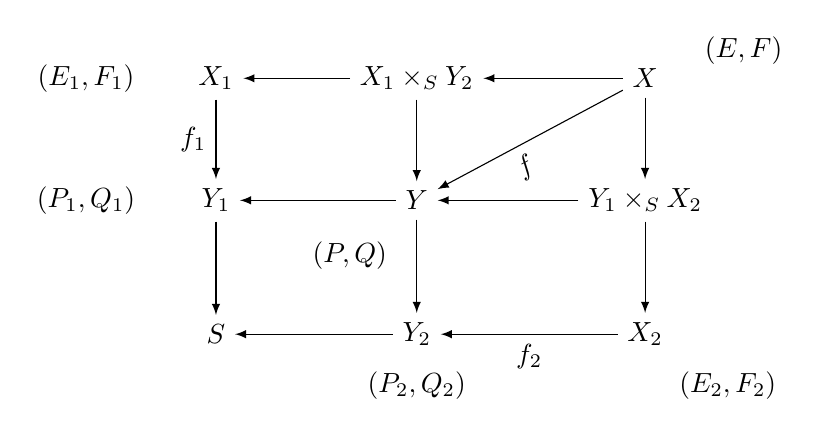
\begin{tikzpicture}[>=latex,baseline=(current bounding box.center)]
\node (EF1) at (-5.2,2.0) {$(E_1,F_1)$};
\node (X1)  at (-3.55,2.0) {$X_1$};
\node (X1Y2) at (-1.0,2.0) {$X_1\times_S Y_2$};
\node (X) at (1.9,2.0) {$X$};
\node (EF) at (3.15,2.35) {$(E,F)$};
\node (PQ1) at (-5.2,0.45) {$(P_1,Q_1)$};
\node (Y1) at (-3.55,0.45) {$Y_1$};
\node (Y) at (-1.0,0.45) {$Y$};
\node (Y1X2) at (1.9,0.45) {$Y_1\times_S X_2$};
\node (S) at (-3.55,-1.25) {$S$};
\node (Y2) at (-1.0,-1.25) {$Y_2$};
\node (X2) at (1.9,-1.25) {$X_2$};
\node (PQ) at (-1.85,-0.25) {$(P,Q)$};
\node (PQ2) at (-1.0,-1.9) {$(P_2,Q_2)$};
\node (EF2) at (2.95,-1.9) {$(E_2,F_2)$};
\draw[->] (X1Y2) -- (X1);
\draw[->] (X) -- (X1Y2);
\draw[->] (X1) -- node[left] {$f_1$} (Y1);
\draw[->] (X1Y2) -- (Y);
\draw[->] (X) -- (Y1X2);
\draw[->] (X) -- node[below,sloped,pos=.58] {$f$} (Y);
\draw[->] (Y) -- (Y1);
\draw[->] (Y1X2) -- (Y);
\draw[->] (Y1) -- (S);
\draw[->] (Y) -- (Y2);
\draw[->] (Y1X2) -- (X2);
\draw[->] (Y2) -- (S);
\draw[->] (X2) -- node[below] {$f_2$} (Y2);
\end{tikzpicture}}
\end{equation}
给定 $(u_1,v_1)\in\Hom_{f_1}^{(3,4)}((E_1,F_1),(P_1,Q_1))$、$(u_2,v_2)\in\Hom_{f_2}^{(2,1)}((E_2,F_2),(P_2,Q_2))$（记号见 2.1.2 和 1.4）。由 1.8，利用 $(u_i,v_i)$ 得到方块
\begin{equation}\tag{2.4.1}
\begin{tikzcd}[column sep=huge,row sep=large]
(E,F) \arrow[d,"{(u_1\otimes^L_S E_2,\,v_1\otimes^L_S F_2)}"] & (E_1\otimes^L_S P_2,F_1\otimes^L_S Q_2) \arrow[l,"{(E_1\otimes^L_S u_2,\,F_1\otimes^L_S v_2)}"'] \arrow[d,"{(u_1\otimes^L_S P_2,\,v_1\otimes^L_S Q_2)}"]\\
(P_1\otimes^L_S E_2,Q_1\otimes^L_S F_2) \arrow[r,"{(P_1\otimes^L_S u_2,\,Q_1\otimes^L_S v_2)}"'] & (P,Q),
\end{tikzcd}
\end{equation}
其中竖直箭头（相应地水平箭头）的类型为 $(3,4)$（相应地 $(2,1)$）。

现在可以陈述本节主要的相容性，它将在验证 Lefschetz--Verdier 公式时起关键作用。

\subsection*{命题 2.5}
下图 2.5.1 交换，其中右边的方块由 2.4.1 按 2.1.3 和 2.1.5 的意义应用 $\RHom$ 而得：
\begin{equation}\tag{2.5.1}
\resizebox{0.98\textwidth}{!}{%
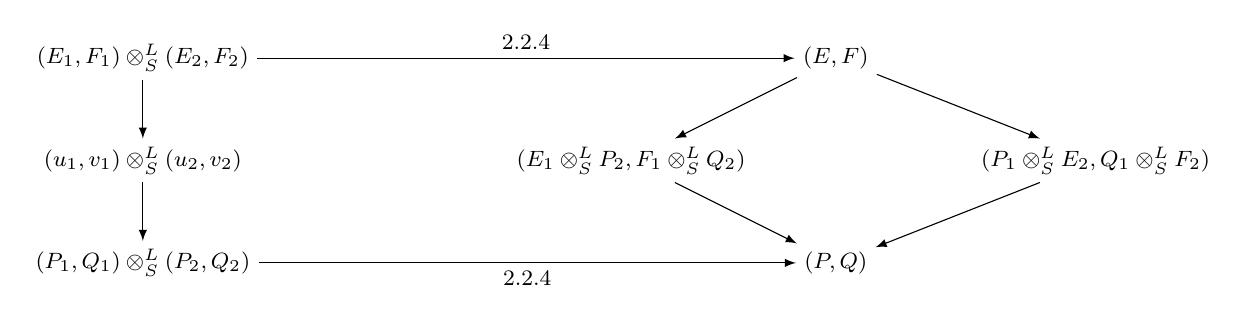
\begin{tikzpicture}[>=latex,baseline=(current bounding box.center)]
\footnotesize
\node (A) at (0,2.6) {$\RHom(E_1,F_1)\otimes^L_S\RHom(E_2,F_2)$};
\node (B) at (0,1.3) {$\RHom(u_1,v_1)\otimes^L_S\RHom(u_2,v_2)$};
\node (C) at (0,0) {$\RHom(P_1,Q_1)\otimes^L_S\RHom(P_2,Q_2)$};
\node (D) at (8.8,2.6) {$\RHom(E,F)$};
\node (E) at (6.2,1.3) {$\RHom(E_1\otimes^L_SP_2,F_1\otimes^L_SQ_2)$};
\node (F) at (12.1,1.3) {$\RHom(P_1\otimes^L_SE_2,Q_1\otimes^L_SF_2)$};
\node (G) at (8.8,0) {$\RHom(P,Q)$};
\draw[->] (A) -- node[above] {$2.2.4$} (D);
\draw[->] (A) -- (B);
\draw[->] (B) -- (C);
\draw[->] (C) -- node[below] {$2.2.4$} (G);
\draw[->] (D) -- (E);
\draw[->] (D) -- (F);
\draw[->] (E) -- (G);
\draw[->] (F) -- (G);
\end{tikzpicture}}
\end{equation}

\subsection*{2.6}
2.5 的证明将占据第~2 节的其余部分。由 1.6.3 可知，若 $w_i:L_i\to M_i$ 是位于 $f_i$ 上的~1 型箭头，则箭头 $w=w_1\otimes^{L}_{S}w_2$ 使下图
\[
\begin{tikzcd}[column sep=large,row sep=large]
& L_1\otimes^L_S L_2 \arrow[dl,"{L_1\otimes^L_S w_2}"'] \arrow[dr,"{w_1\otimes^L_S L_2}"] & \\
L_1\otimes^L_S M_2 \arrow[dr,"{w_1\otimes^L_S M_2}"'] & & M_1\otimes^L_S L_2 \arrow[dl,"{M_1\otimes^L_S w_2}"]\\
& M_1\otimes^L_S M_2 &
\end{tikzcd}
\]
交换。将这一观察应用于 $w_i=\RHom(u_i,v_i)$，可知只需证明 2.5 的下列特例。

\subsection*{推论 2.6.1}
设 $f:X\to Y$ 是 $S$-态射，$S'$ 是 $S$-概形，$f':X'\to Y'$ 是 $f$ 经基变换 $S'\to S$ 导出的态射，$E,F\in\ob D_{\ctf}(X)$，$P,Q\in\ob D_{\ctf}(Y)$，$P',Q'\in\ob D_{\ctf}(S')$，且 $(u,v)\in\Hom_f^{(2,1)}((E,F),(P,Q))$（相应地 $\Hom_f^{(3,4)}((E,F),(P,Q))$）。则有一个交换方块，其竖直箭头是位于 $f'$ 上的~1 型箭头：
\begin{equation}\tag{2.6.1.1}
\begin{tikzcd}[column sep=large,row sep=large]
\RHom(E,F)\otimes^L_S\RHom(P',Q') \arrow[r,"2.2.4"] \arrow[d,"{\RHom(u,v)\otimes^L_S\RHom(P',Q')}"'] & \RHom(E\otimes^L_SP',F\otimes^L_SQ') \arrow[d,"{\RHom(u\otimes^L_SP',v\otimes^L_SQ')}"]\\
\RHom(P,Q)\otimes^L_S\RHom(P',Q') \arrow[r,"2.2.4"'] & \RHom(P\otimes^L_SP',Q\otimes^L_SQ').
\end{tikzcd}
\end{equation}
先考察 $(u,v)$ 为 $(2,1)$ 型的情形。由函子性，可设 $E=f^{*}P$、$F=f^{*}Q$，且 $(u,v)$ 由 $(f^{*}P,f^{*}Q)$ 的恒等态射给出。当 $P'=Q'=A_{S'}$ 时，2.6.1.1 的交换性显然；因此，要证明一般情形，只需验证对 $L,M\in\ob D_{\ctf}(Y)$，方块
\[
\begin{tikzcd}[column sep=large,row sep=large]
f^{*}\RHom(E,F)\otimes^L f^{*}\RHom(L,M) \arrow[r,"{f^*(2.2.3)}"] \arrow[d,"{2.1.1\otimes 2.1.1}"'] & f^{*}\RHom(E\otimes^LL,F\otimes^LM) \arrow[d,"2.1.1"]\\
\RHom(f^{*}E,f^{*}F)\otimes^L\RHom(f^{*}L,f^{*}M) \arrow[r,"2.2.3"'] & \RHom(f^{*}(E\otimes^LL),f^{*}(F\otimes^LM))
\end{tikzcd}
\]
交换。但立即可见，该方块的两个复合都与求值箭头
\[
f^{*}E\otimes^L f^{*}\RHom(E,F)\longrightarrow f^{*}F
\quad\text{且}\quad
f^{*}L\otimes^L f^{*}\RHom(L,M)\longrightarrow f^{*}M,
\]
的张量积伴随，从而证明了所述断言。

现在转向 $(u,v)$ 为 $(3,4)$ 型的情形。由函子性，可设 $P=f_{!}E$、$F=f^{!}Q$，且 $(u,v)$ 由 $(\Id_P,\Id_F)$ 定义。须证明下列方块交换
\[
\begin{tikzcd}[column sep=large,row sep=large]
f_*\RHom(E,f^!Q)\otimes^L_S\RHom(P',Q') \arrow[r,"b"] \arrow[d,"{a\otimes^L_S\RHom(P',Q')}"'] & f'_*\RHom(E\otimes^L_SP',f^!Q\otimes^L_SQ') \arrow[d,"a'"]\\
\RHom(f_!E,Q)\otimes^L_S\RHom(P',Q') \arrow[r,"2.2.4"'] & \RHom(f_!E\otimes^L_SP',Q\otimes^L_SQ'),
\end{tikzcd}
\]
其中 $b$ 是 $f'_*(2.2.4)$ 与一个基变换同构的复合，$a$ 是对偶同构（SGA~4~XVIII~3.1.9.6），$a'$ 则是关于 $E\otimes^L_SP'$、$Q\otimes^L_SQ'$ 的对偶同构与基变换同构
\[
f_!E\otimes^L_SP'\xrightarrow[\sim]{c}f'_!(E\otimes^L_SP'),
\qquad
f^!Q\otimes^L_SQ'\xrightarrow[\sim]{d}f'^!(Q\otimes^L_SQ').
\]
的复合。回顾 $a$ 是典范箭头（SGA~4~XVIII~3.1.9.5）
\[
f_*\RHom(E,f^!Q)\longrightarrow\RHom(f_!E,f_!f^!Q)
\]
与由伴随箭头 $f_!f^!Q\to Q$ 定义的箭头的复合。$a'$ 也有类似描述，即将上述箭头
\begin{equation}\tag{*}
f'_*\RHom(E\otimes^L_SP',f^!Q\otimes^L_SQ')\longrightarrow
\RHom(f'_!(E\otimes^L_SP'),f'_!(f^!Q\otimes^L_SQ')),
\end{equation}
与由 $c$、$d$ 定义的箭头，以及由伴随箭头
\[
f'_!f'^!(Q\otimes^L_SQ')\longrightarrow Q\otimes^L_SQ'.
\]
定义的箭头复合。按照定义，$d$ 与由基变换同构 $f'_!(f^!Q\otimes^L_SQ')\simeq f_!f^!Q\otimes^L_SQ'$ 和伴随箭头 $f_!f^!Q\to Q$ 定义的箭头
\[
f'_!(f^!Q\otimes^L_SQ')\longrightarrow Q\otimes^L_SQ'
\]
伴随；换言之，方块
\[
\begin{tikzcd}[column sep=large,row sep=large]
f'_!(f^!Q\otimes^L_SQ') \arrow[r,"{f'_!d}"] \arrow[d,"{\text{基变换}\ \sim}"'] & f'_!f'^!(Q\otimes^L_SQ') \arrow[d,"\mathrm{adj}"]\\
f_!f^!Q\otimes^L_SQ' \arrow[r,"{\mathrm{adj}\otimes 1}"'] & Q\otimes^L_SQ'
\end{tikzcd}
\]
交换。因此也可将 $a'$ 描述为 (*)、由 $c$ 定义的箭头、以及由基变换同构
\[
f'_!(f^!Q\otimes^L_SQ')\xrightarrow{\sim}f_!f^!Q\otimes^L_SQ'
\]
和伴随箭头 $f_!f^!Q\to Q$ 定义的箭头的复合。$a'$ 的这一分解及上面给出的 $a$ 的分解，加上下列方块
\[
\begin{tikzcd}[column sep=large,row sep=large]
\RHom(f_!E,f_!f^!Q)\otimes^L_S\RHom(P',Q') \arrow[r] \arrow[d] & \RHom(f_!E\otimes^L_SP',f_!f^!Q\otimes^L_SQ') \arrow[d]\\
\RHom(f_!E,Q)\otimes^L_S\RHom(P',Q') \arrow[r] & \RHom(f_!E\otimes^L_SP',Q\otimes^L_SQ'),
\end{tikzcd}
\]
（由 2.2.4 和伴随箭头 $f_!f^!Q\to Q$ 定义）的交换性，说明要证明 2.6.2 交换，只需证明下列相容性。

\subsection*{引理 2.6.3}
设 $f$、$f'$、$E$、$F$、$P'$、$Q'$ 同 2.6.1。则有交换方块
\[
\begin{tikzcd}[column sep=large,row sep=large]
f_*\RHom(E,F)\otimes^L_S\RHom(P',Q') \arrow[r,"(1)"] \arrow[d,"(2)"'] & f'_*\RHom(E\otimes^L_SP',F\otimes^L_SQ') \arrow[d,"(4)"]\\
\RHom(f_!E,f_!F)\otimes^L_S\RHom(P',Q') \arrow[r,"(3)"'] & \RHom(f_!E\otimes^L_SP',f_!F\otimes^L_SQ'),
\end{tikzcd}
\]
其中 (1) 是基变换同构
\[
f_*\RHom(E,F)\otimes^L_S -\xrightarrow{\sim}f'_*\bigl(\RHom(E,F)\otimes^L_S-\bigr)
\]
与 $f'_*(2.2.4)$ 的复合，(2) 是对典范箭头
\[
f_*\RHom(E,F)\longrightarrow\RHom(f_!E,f_!F)
\]
（SGA~4~XVIII~3.1.9.5）应用 $\otimes^L_S\RHom(P',Q')$ 得到的，(3) 由 2.2.4 给出，最后，(4) 是典范箭头
\[
f'_*\RHom(E\otimes^L_SP',F\otimes^L_SQ')
\longrightarrow
\RHom(f'_!(E\otimes^L_SP'),f'_!(F\otimes^L_SQ'))
\]
（见所引文献）与由基变换同构
\[
f'_!(E\otimes^L_SP')\xrightarrow{\sim}f_!E\otimes^L_SP',
\qquad
f'_!(F\otimes^L_SQ')\xrightarrow{\sim}f_!F\otimes^L_SQ'.
\]
回到箭头（SGA~4~XVIII~3.1.9.5）的定义，选择 $f$ 的一个紧化\footnote{上述箭头借助这样的紧化定义，但不依赖它：这一点在所引文献中被默认为真，其实很容易验证。}，于是只需分别在 $f$ 为开浸入和 $f$ 为固有态射时证明引理。

\emph{a) $f$ 为开浸入的情形。} 由伴随（2.2.1），只需说明，将方块 2.6.3 与 $f_!E\otimes^L_SP'$ 作张量积，再与求值箭头 2.2.2
\[
(f_!E\otimes^L_SP')\otimes^L\RHom(f_!E\otimes^L_SP',f_!F\otimes^L_SQ')\longrightarrow f_!F\otimes^L_SQ',
\]
复合后，所得方块交换。但该方块各项在 $X'$ 以外都为零，故只需验证其在 $X'$ 上诱导的方块交换，而这是平凡的。

\emph{b) $f$ 为固有态射的情形。} 此时 $f_!=f_*$、$f'_!=f'_*$。容易看出，将
\[
f_*\RHom(E,F)\longrightarrow\RHom(f_*E,f_*F)
\]
与平凡对偶同构
\[
\RHom(f_*E,f_*F)\xrightarrow{\sim}f_*\RHom(f^{*}f_*E,F)
\]
（2.1.4）复合，所得正是由伴随箭头 $f^{*}f_*E\to E$ 应用 $f_*\RHom(-,F)$ 导出的箭头。类似地，将 (4) 与平凡对偶同构
\[
\RHom(f_*E\otimes^L_SP',f_*F\otimes^L_SQ')\xrightarrow{\sim}f'_*\RHom(f^{*}f_*E\otimes^L_SP',F\otimes^L_SQ')
\]
复合（其中由典范同构将 $f_*F\otimes^L_SQ'$ 与 $f'_*(F\otimes^L_SQ')$ 认同），所得正是由伴随箭头 $f^{*}f_*E\to E$ 应用 $f'_*\RHom(-\otimes^L_SP',F\otimes^L_SQ')$ 导出的箭头。因此只需验证下列方块的交换性
\[
\begin{tikzcd}[column sep=large,row sep=large]
\RHom(f_*E,f_*F)\otimes^L_S\RHom(P',Q') \arrow[r,"(3)"] \arrow[d] & \RHom(f_*E\otimes^L_SP',f_*F\otimes^L_SQ') \arrow[d]\\
f_*\RHom(f^{*}f_*E,F)\otimes^L_S\RHom(P',Q') \arrow[r,"(1')"'] & f'_*\RHom(f^{*}f_*E\otimes^L_SP',F\otimes^L_SQ'),
\end{tikzcd}
\]
其中竖直箭头是平凡对偶同构，$(1')$ 则由 (1) 将 $E$ 换成 $f^{*}f_*E$ 而得。但这是已处理的 $(u,v)$ 为 $(2,1)$ 型时 2.6.1.1 的一个特例（取由 $f^{*}f_*E$ 的恒等态射给出的 $u:f^{*}f_*E\to f_*E$，以及由 $f_*F$ 的恒等态射给出的 $v:F\to f_*F$）。至此证明了 2.6.3。如前所述，2.6.2 的交换性随之成立，从而完成了 2.6.1、最终也完成了 2.5 的证明。

\clearpage
\section{上同调对应}

\subsection*{3.1}
对 $i=1,2$，设 $X_i$ 是 $S$-概形，$L_i\in\ob\Dctf(X_i)$，并设
\[
X=X_1\times_S X_2,
\qquad
p_i:X\longrightarrow X_i,
\qquad
q_i:X_i\longrightarrow S
\]
是典范投影：
\[
\begin{tikzcd}[column sep=1.8em,row sep=1.5em]
& X \arrow[dl,"P_1"'] \arrow[dr,"P_2"] & \\
L_1\quad X_1 \arrow[dr,"q_1"'] & & X_2\quad L_2 \arrow[dl,"q_2"] \\
& S &
\end{tikzcd}
\]
采用 1.3 的记号，有典范同构（2.2.4）
\[
DL_1\overset{\mathbf L}{\otimes}_S L_2
\xrightarrow{\sim}
\RHom\bigl(L_1\overset{\mathbf L}{\otimes}_S A_{X_2},
q_1^!A_S\overset{\mathbf L}{\otimes}_S L_2\bigr).
\]
再与 Künneth 同构
\[
q_1^!A_S\overset{\mathbf L}{\otimes}_S L_2
\xrightarrow{\sim}p_2^!L_2 \qquad (1.7.3),
\]
复合，得到同构
\begin{equation}
DL_1\overset{\mathbf L}{\otimes}_S L_2
\xrightarrow{\sim}
\RHom(p_1^*L_1,p_2^!L_2).
\tag{3.1.1}
\end{equation}
这一同构在全文中起基础作用。当 $X_i=S$ 时，3.1.1 化为
\[
L_1^\vee\overset{\mathbf L}{\otimes}L_2\xrightarrow{\sim}\RHom(L_1,L_2),
\]
这是任意赋环拓扑斯上完美复形所具有的同构（SGA 6 I 7.7）的一个特例。令
\begin{equation}
\RHom(p_1^*L_1,p_2^!L_2)=\RHom_S(L_1,L_2),
\qquad
\Hom(p_1^*L_1,p_2^!L_2)=\Hom_S(L_1,L_2).
\tag{3.1.2}
\end{equation}
称 $\Hom_S(L_1,L_2)$ 的元素为\emph{从 $L_1$ 到 $L_2$ 的上同调对应}。将“从 $A_{X_1}$ 到 $A_{X_2}$ 的上同调对应”简称为\emph{从 $X_1$ 到 $X_2$ 的上同调对应}（系数默认为 $A$）。

若 $X_1$ \emph{光滑}且纯相对维数为 $r_1$，则 $p_2$ 也具有此性质，由对偶定理（SGA 4 XVIII 3.2.5）有
\[
p_2^!L_2\xrightarrow{\sim}p_2^*L_2(r_1)[2r_1],
\]
因此
\begin{equation}\begin{gathered}
\RHom_S(L_1,L_2)=\RHom(p_1^*L_1,p_2^*L_2)(r_1)[2r_1],
\\
\Hom_S(L_1,L_2)=\H^{2r_1}\bigl(X,\RHom(p_1^*L_1,p_2^*L_2)(r_1)\bigr).
\tag{3.1.3}
\end{gathered}\end{equation}
特别地，此时从 $X_1$ 到 $X_2$ 的上同调对应群与 $\H^{2r_1}(X,A(r_1))$ 认同。

\subsection*{3.2}
实际遇到的上同调对应与 $S$-态射 $X_2\to X_1$ 相联系，或者更一般地与 $X$ 上的圈或 $X$ 上方的概形相联系。设
\[
c:C\longrightarrow X
\]
是 $X$ 上方的概形（有时也称 $c$ 为 $X_1$ 与 $X_2$ 之间的一个对应），并记投影为 $c_i=p_ic:C\to X_i$。称群
\[
\H^0\bigl(X,c_!\RHom(c_1^*L_1,c_2^!L_2)\bigr)
\quad(=\Hom(c_1^*L_1,c_2^!L_2)\text{，若 }c\text{ 固有}).
\]
的元素为\emph{从 $L_1$ 到 $L_2$、支集在 $c$ 中的上同调对应}（无混淆之虞时也说支集在 $C$ 中）。由诱导公式（SGA 4 XVIII 3.1.12.2），有典范同构
\begin{equation}
c^!\RHom(p_1^*L_1,p_2^!L_2)
\xrightarrow{\sim}
\RHom(c_1^*L_1,c_2^!L_2),
\tag{3.2.1}
\end{equation}
因此，应用 $c_!$ 并与伴随箭头 $c_!c^!\to \Id$ 复合，得到典范箭头
\begin{equation}
c_!\RHom(c_1^*L_1,c_2^!L_2)
\longrightarrow
\RHom(p_1^*L_1,p_2^!L_2),
\tag{3.2.2}
\end{equation}
\begin{equation}
\H^0\bigl(X,c_!\RHom(c_1^*L_1,c_2^!L_2)\bigr)
\longrightarrow
\Hom_S(L_1,L_2).
\tag{3.2.3}
\end{equation}
所以，每个从 $L_1$ 到 $L_2$、支集在 $C$ 中的对应，都通过 3.2.3 典范地定义一个从 $L_1$ 到 $L_2$ 的（不指定支集的）对应。

\emph{例。} a) 设 $c$ 固有，且 $c_2$ 具有有限 Tor 维数，相对维数 $\leq N$。迹态射（SGA $4^{1/2}$，圈 2.3.3）
\[
\mathrm{Tr}_{c_2}:c_{2!}A_C\longrightarrow A_{X_2}(-N)[-2N]
\]
通过伴随定义一个从 $A_{X_1}$ 到 $A_{X_2}(-N)[2N]$、支集在 $C$ 中的上同调对应，称为 \emph{$(c,N)$ 的类}，记作
\begin{equation}
\operatorname{cl}(c,N)\in \H^{-2N}\bigl(C,c_2^!A_{X_2}(-N)\bigr).
\tag{3.2.4}
\end{equation}
最重要的是 $N=0$ 的情形，即 $c_2$ 有限（且有有限 Tor 维数）；此时 $\operatorname{cl}(c)$ 是从 $X_1$ 到 $X_2$、支集在 $C$ 中的上同调对应。若 $X_1$ 光滑且纯相对维数为 $r_1$，则由 3.1.3 和 3.2.1，
\begin{equation}
\H^{-2N}\bigl(C,c_2^!A_{X_2}(-N)\bigr)
=
\H^{2(r_1-N)}\bigl(C,c^!A_X(r_1-N)\bigr).
\tag{3.2.5}
\end{equation}
若进一步 $c$ 是闭浸入，右端可写为
\[
\H^{2(r_1-N)}_C\bigl(X,A_X(r_1-N)\bigr),
\]
而将 $(c,N)$ 的类视为该群的元素时，它恰好就是（SGA $4^{1/2}$，圈 2.3.1）意义下与 $c$ 相联系的上同调类；这直接由定义可得。

b) 设 $F:X_2\to X_1$ 是 $S$-态射，用 $c(F):C(F)\to X$ 表示其图像，即由 $F$ 定义的 $p_2$ 的截面的像（“点 $(Fx,x)$ 构成的集合”）：$c_2$ 是同构，且 $c_1c_2^{-1}=F$。于是有典范同构
\begin{equation}\begin{gathered}
\RHom\bigl(c_1(F)^*L_1,c_2(F)^!L_2\bigr)=\RHom(F^*L_1,L_2),
\\
\Hom\bigl(c_1(F)^*L_1,c_2(F)^!L_2\bigr)=\Hom(F^*L_1,L_2).
\tag{3.2.6}
\end{gathered}\end{equation}
换言之，从 $L_1$ 到 $L_2$、支集在 $F$ 的图像中的上同调对应，正是将 $F$ “提升”为同态 $F^*L_1\to L_2$ 所得的对象。以下是两个重要的例子：

(i) $X_1=X_2$，$L_1=L_2$，$F=1$ 是 $X_1$ 的恒等态射，其图像 $\Delta$ 是对角线。由 $L_1$ 的恒等态射定义的支集在 $\Delta$ 中的对应，称为\emph{对角对应}。它就是元素
\[
1\in \Hom(L_1,L_1)=\H^0\bigl(X,\Delta_*\Delta^!\RHom_S(L_1,L_1)\bigr)
\]
（若 $X_1$ 光滑且纯相对维数为 $r$，则此群与 $\H^{2r}_\Delta(X,\RHom_S(L_1,L_1)(r))$ 认同）。

(ii) 设 $S$ 是有限域 $\mathbb F_q$ 的谱，$X_1=X_2$，$L_1=L_2$，取 $F:X_1\to X_1$ 为 $\mathbb F_q$ 上的相对 Frobenius 自同态，即在底空间上为恒等、在 $\mathcal O_{X_1}$ 上取 $q$ 次幂的自同态（参见 XIV），并取 $F$ 到 $L_1$ 的提升为典范同构
\[
F^*L_1\xrightarrow{\sim}L_1
\]
（所引文献第~2 节命题 1）（更准确地说，若 $q=p^a$，则取所引文献中同构的 $a$ 次迭代）。由此定义的从 $L_1$ 到 $L_1$、支集在 $F$ 的图像中的上同调对应，称为（关于 $\mathbb F_q$ 的）\emph{Frobenius 对应}。

c) Langlands 在（[13] 第~7 节）研究了与 Hecke 算子有关的某些曲线上层之间的上同调对应。

d) 常层之间的上同调对应（自然出现得最多的情形）通过“积分”自然给出复形之间的上同调对应，下面即说明这一点。

\subsection*{3.3}
对 $i=1,2$，设 $f_i:X_i\to Y_i$ 是 $S$-态射，并令
\[
f=f_1\times_S f_2:X\to Y,
\qquad
f'_1=f_1\times_S Y_2,
\qquad
f'_2=Y_1\times_S f_2,
\]
\[
p'_1=X_1\times_S f_2,
\qquad
p'_2=f_1\times_S X_2.
\]
\begin{equation}
\begin{tikzcd}[column sep=3.8em,row sep=2.4em]
X_1\times_S Y_2 \arrow[d,"f'_1"'] & X \arrow[l,"p'_1"'] \arrow[dl,"f" description] \arrow[d,"p'_2"] \\
Y & Y_1\times_S X_2 \arrow[l,"f'_2"]
\end{tikzcd}
\tag{3.3.0}
\end{equation}
设 $L_i\in\ob\Dctf(X_i)$。存在唯一同构
\begin{equation}
f_*\RHom_S(L_1,L_2)
\xrightarrow{\sim}
\RHom_S(f_{1!}L_1,f_{2*}L_2)
\tag{3.3.1}
\end{equation}
其逆使下列方块
\[
\begin{tikzcd}[column sep=4.5em,row sep=2.6em]
D(f_{1!}L_1)\overset{\mathbf L}{\otimes}_S f_{2*}L_2
  \arrow[r,"3.1.1"] \arrow[d,"(1)"']
& \RHom_S(f_{1!}L_1,f_{2*}L_2) \arrow[d] \\
f_{1*}DL_1\overset{\mathbf L}{\otimes}_S f_{2*}L_2
  \arrow[r,"(2)"']
& f_*\RHom_S(L_1,L_2),
\end{tikzcd}
\]
交换，其中 (1) 由对偶同构（SGA 4 XVIII 3.1.9.6）
\[
Df_{1!}L_1\xrightarrow{\sim}f_{1*}DL_1
\]
的逆应用 $-\overset{\mathbf L}{\otimes}_S f_{2*}L_2$ 而得，(2) 则是 Künneth 同构
\[
f_{1*}DL_1\overset{\mathbf L}{\otimes}_S f_{2*}L_2
\xrightarrow{\sim}
f_*(DL_1\overset{\mathbf L}{\otimes}_S L_2)
\]
与 $f_*(3.1.1)$ 的复合。对 3.3.1 应用 $R\Gamma(Y,-)$，得到同构
\begin{equation}
f_*:\Hom_S(L_1,L_2)
\xrightarrow{\sim}
\Hom_S(f_{1!}L_1,f_{2*}L_2).
\tag{3.3.2}
\end{equation}
对 $u\in\Hom_S(L_1,L_2)$，称对应 $f_*u$ 为 $u$ 沿 $f$ 的\emph{正像}。当 $Y_1=Y_2=S$ 时，将 $f_*u$ 记作 $u_*$。若 $Y_1=Y_2=S$ 是可分闭域的谱，则 3.3.2 写为
\begin{equation}
\Hom_S(L_1,L_2)
\xrightarrow{\sim}
\Hom\bigl(R\Gamma_c(X_1,L_1),R\Gamma(X_2,L_2)\bigr).
\tag{3.3.3}
\end{equation}
因此，上同调对应在上同调上“作用”。以下陈述给出这一作用的几种解释，尤其将它与上述 a)、b) 等情形中的通常定义联系起来。

\begin{statement}{命题 3.4}
采用 3.3.0 的记号，在 $\Dctf(Y)$ 中有下列由同构构成的交换图：
\begin{equation}
\begin{tikzcd}[column sep=4.0em,row sep=2.8em]
& \RHom_S(f_{1!}L_1,f_{2*}L_2)
  \arrow[dl,"(1)"'] \arrow[dr,"(2)"] \arrow[dd,"(5)" description] & \\
f'_{1*}\RHom_S(L_1,f_{2*}L_2) \arrow[dr,"f'_{1*}(3)"'] &&
f'_{2*}\RHom_S(f_{1!}L_1,L_2) \arrow[dl,"f'_{2*}(4)"] \\
& f_*\RHom_S(L_1,L_2) &
\end{tikzcd}
\tag{3.4.1}
\end{equation}
其中 (5) 是 3.3.1 的逆，箭头 (1) 至 (4) 由下列交换图定义；图中“基变换”表示由第~1 节所考虑类型的基变换或 Künneth 同构导出的箭头，“对偶”表示由 2.1.4 型或（SGA 4 XVIII 3.1.9.6）型对偶同构导出的箭头，“平凡”表示平凡同构：
\[
\begin{tikzcd}[column sep=3.7em,row sep=1.7em]
\RHom(f_{1!}L_1\overset{\mathbf L}{\otimes}_S A_{Y_2},K_{Y_1}\overset{\mathbf L}{\otimes}_S f_{2*}L_2)
  \arrow[r,"\text{基变换}"] \arrow[d,"\text{基变换}"']
& \RHom_S(f_{1!}L_1,f_{2*}L_2) \arrow[ddd,"(1)"] \\
\RHom(f'_{1!}(L_1\overset{\mathbf L}{\otimes}_S A_{Y_2}),K_{Y_1}\overset{\mathbf L}{\otimes}_S f_{2*}L_2) \arrow[d,"\text{对偶}"']
& \\
f'_{1*}\RHom(L_1\overset{\mathbf L}{\otimes}_S A_{Y_2},f_1'^!(K_{Y_1}\overset{\mathbf L}{\otimes}_S f_{2*}L_2)) \arrow[d,"\text{基变换}"']
& \\
f'_{1*}\RHom(L_1\overset{\mathbf L}{\otimes}_S A_{Y_2},K_{X_1}\overset{\mathbf L}{\otimes}_S f_{2*}L_2) \arrow[r,"\text{基变换}"']
& f'_{1*}\RHom_S(L_1,f_{2*}L_2),
\end{tikzcd}
\]
\[
\begin{tikzcd}[column sep=3.7em,row sep=1.7em]
\RHom(f_{1!}L_1\overset{\mathbf L}{\otimes}_S A_{Y_2},K_{Y_1}\overset{\mathbf L}{\otimes}_S f_{2*}L_2)
  \arrow[r,"\text{基变换}"] \arrow[d,"\text{基变换}"']
& \RHom_S(f_{1!}L_1,f_{2*}L_2) \arrow[ddd,"(2)"] \\
\RHom(f_{1!}L_1\overset{\mathbf L}{\otimes}_S A_{Y_2},f'_{2*}(K_{Y_1}\overset{\mathbf L}{\otimes}_S L_2)) \arrow[d,"\text{对偶}"']
& \\
f'_{2*}\RHom(f_2'^*(f_{1!}L_1\overset{\mathbf L}{\otimes}_S A_{Y_2}),K_{Y_1}\overset{\mathbf L}{\otimes}_S L_2) \arrow[d,"\text{平凡}"']
& \\
f'_{2*}\RHom(f_{1!}L_1\overset{\mathbf L}{\otimes}_S A_{X_2},K_{Y_1}\overset{\mathbf L}{\otimes}_S L_2) \arrow[r,"\text{基变换}"']
& f'_{2*}\RHom_S(f_{1!}L_1,L_2),
\end{tikzcd}
\]
\[
\begin{tikzcd}[column sep=3.7em,row sep=1.7em]
\RHom(L_1\overset{\mathbf L}{\otimes}_S A_{Y_2},K_{X_1}\overset{\mathbf L}{\otimes}_S f_{2*}L_2)
  \arrow[r,"\text{基变换}"] \arrow[d,"\text{基变换}"']
& \RHom_S(L_1,f_{2*}L_2) \arrow[ddd,"(3)"] \\
\RHom(L_1\overset{\mathbf L}{\otimes}_S A_{Y_2},p'_{1*}(K_{X_1}\overset{\mathbf L}{\otimes}_S L_2)) \arrow[d,"\text{对偶}"']
& \\
p'_{1*}\RHom(p_1'^*(L_1\overset{\mathbf L}{\otimes}_S A_{Y_2}),K_{X_1}\overset{\mathbf L}{\otimes}_S L_2) \arrow[d,"\text{平凡}"']
& \\
p'_{1*}\RHom(L_1\overset{\mathbf L}{\otimes}_S A_{X_2},K_{X_1}\overset{\mathbf L}{\otimes}_S L_2) \arrow[r,"\text{基变换}"']
& p'_{1*}\RHom_S(L_1,L_2),
\end{tikzcd}
\]
\[
\begin{tikzcd}[column sep=3.7em,row sep=1.7em]
\RHom(f_{1!}L_1\overset{\mathbf L}{\otimes}_S A_{X_2},K_{Y_1}\overset{\mathbf L}{\otimes}_S L_2)
  \arrow[r,"\text{基变换}"] \arrow[d,"\text{基变换}"']
& \RHom_S(f_{1!}L_1,L_2) \arrow[ddd,"(4)"] \\
\RHom(p'_{2!}(L_1\overset{\mathbf L}{\otimes}_S A_{X_2}),K_{Y_1}\overset{\mathbf L}{\otimes}_S L_2) \arrow[d,"\text{对偶}"']
& \\
p'_{2*}\RHom(L_1\overset{\mathbf L}{\otimes}_S A_{X_2},p_2'^!(K_{Y_1}\overset{\mathbf L}{\otimes}_S L_2)) \arrow[d,"\text{基变换}"']
& \\
p'_{2*}\RHom(L_1\overset{\mathbf L}{\otimes}_S A_{X_2},K_{X_1}\overset{\mathbf L}{\otimes}_S L_2) \arrow[r,"\text{基变换}"']
& p'_{2*}\RHom_S(L_1,L_2).
\end{tikzcd}
\]
\end{statement}
这只是将 2.5 在以下特例中展开：$(u_1,v_1):(L_1,K_{X_1})\to(f_{1!}L_1,K_{Y_1})$ 由 $f_{1!}L_1$ 的恒等态射及典范同构 $f_1^!K_{Y_1}\xrightarrow{\sim}K_{X_1}$ 给出，而 $(u_2,v_2):(A_{X_2},L_2)\to(A_{Y_2},f_{2*}L_2)$ 由典范同构 $A_{X_2}\xrightarrow{\sim}f_2^!A_{Y_2}$ 及 $f_{2*}L_2$ 的恒等态射给出。

\begin{statement}{推论 3.5}
设 $Y_1=Y_2=S$。给定 $u\in\Hom_S(L_1,L_2)$，正像 $f_*u\in\Hom(f_{1!}L_1,f_{2*}L_2)$（3.3.2）可由下列两种等价方式得到：
\end{statement}
\begin{enumerate}[label=\alph*)]
\item 利用平凡对偶，将 $u$ 与一个箭头
\[
L_1\longrightarrow p_{1*}p_2^!L_2;
\]
认同；再与基变换同构
\[
p_{1*}p_2^!L_2\xrightarrow{\sim}f_1^!f_{2*}L_2;
\]
复合，$f_*u$ 就是此复合箭头的伴随箭头。
\item 利用伴随，将 $u$ 与一个箭头
\[
p_{2!}p_1^*L_1\longrightarrow L_2;
\]
认同；再与基变换同构
\[
f_2^*f_{1!}L_1\xrightarrow{\sim}p_{2!}p_1^*L_1;
\]
复合，$f_*u$ 就是此复合箭头的伴随箭头。
\end{enumerate}
描述 a)（相应地 b)）确实对应于 3.4.1 中的路径 $(f_{1*}(3)\circ(1))^{-1}$（相应地 $f_{2*}(4)\circ(2)$）。

\subsection*{3.6}
实际中主要使用描述 3.5 b)。下面在上同调类的层面将它展开；为简化记号，设 $S$ 是可分闭域的谱。给定
\[
u\in\Hom_S(L_1,L_2)=\Hom(p_1^*L_1,p_2^!L_2).
\]
对 $x\in\allowbreak \H_c^i(X_1,L_1)$，$u_*(x)\in\allowbreak \H^i(X_2,L_2)$ 定义如下：考虑由 $x$ 取逆像得到的元素 $p_1^*x\in\allowbreak \H^i(X_2,p_{2!}p_1^*L_1)$，对其应用 $u$，即取乘积
\[
u\cdot p_1^*x\in \H^i(X_2,p_{2!}p_2^!L_2),
\]
然后应用由伴随箭头 $p_{2!}p_2^!\to\Id$ 定义的箭头
\[
a:\H^i(X_2,p_{2!}p_2^!L_2)\longrightarrow \H^i(X_2,L_2)
\]
即可；简言之：
\begin{equation}
u_*(x)=a(u\cdot p_1^*x).
\tag{3.6.1}
\end{equation}
设 $c:C\to X$ 是固有态射，$u\in\Hom(c_1^*L_1,c_2^!L_2)$。用
\[
u_*\in\Hom\bigl(R\Gamma_c(X_1,L_1),R\Gamma(X_2,L_2)\bigr)
\]
表示 $u$ 在 3.2.3 与 3.3.3 的复合下的像。由 3.6.1 可知，对 $x\in\H_c^i(X_1,L_1)$，有
\begin{equation}
u_*(x)=a(u\cdot c_1^*x),
\tag{3.6.2}
\end{equation}
其中 $c_1^*x$ 是 $x$ 在 $\H^i(X_2,c_{2!}c_1^*L_1)$ 中的逆像，而
\[
a:\H^i(X_2,c_{2!}c_2^!L_2)\longrightarrow \H^i(X_2,L_2)
\]
是由伴随 $c_{2!}c_2^!L_2\to\Id$ 导出的箭头。在例 3.2 a) 的情形中，由此得到
\begin{equation}
\operatorname{cl}(c,N)_*(x)=\mathrm{Tr}_{c_2}(c_1^*x),
\tag{3.6.3}
\end{equation}
其中
\[
\mathrm{Tr}_{c_2}:\H^i(X_2,Rc_{2!}A_C)\longrightarrow\H^{i-2N}(X_2,A(-N))
\]
是关于 $c_2$ 的迹态射诱导的箭头。当 $N=0$ 时，此公式与（SGA $4^{1/2}$，圈 3.6）一致：$\operatorname{cl}(c)_*$ 就是那里记为 $\eta_{X_2,X_1}$ 的同态。若 $X_1$ 光滑且纯相对维数为 $r_1$，$c$ 是闭浸入，则由 3.6.1 及 3.2 a) 末尾的注记，还有
\begin{equation}
\operatorname{cl}(c,N)_*(x)=\mathrm{Tr}_{p_2}(\operatorname{cl}(c)\,p_1^*x),
\tag{3.6.4}
\end{equation}
其中 $\operatorname{cl}(C)\in \H_C^{2(r_1-N)}(X,A(r_1-N))$ 是 $C$ 的上同调类，而
\[
\mathrm{Tr}_{p_2}:\H^*(X_2,Rp_{2!}A_X)\longrightarrow \H^{*-2r_1}(X_2,A(-r_1))
\]
是由关于 $p_2$ 的迹态射定义的箭头。这样便重新得到对应在上同调上诱导同态的通常定义（[12] 1.3）、（SGA $4^{1/2}$，圈 3.2）。

\subsection*{3.6.5}
在 3.2 b) 的情形中，由 3.6.2 可知，对 $u\in\Hom(F^*L_1,L_2)$，
\[
u_*:\H_c^i(X_1,L_1)\longrightarrow \H^i(X_2,L_2)
\]
是“逆像”同态
\[
\H_c^i(X_1,L_1)\longrightarrow \H^i(X_2,F^*L_1)
\]
与 $u$ 诱导的同态的复合（更一般地，$f_*u:Rf_{1!}L_1\to Rf_{2*}L_2$ 是典范同态
\[
Rf_{1!}L_1\longrightarrow Rf_{2*}F^*L_1
\]
与 $Rf_{2*}u$ 的复合）。特别地，对角对应诱导典范箭头
\[
Rf_{1!}L_1\longrightarrow Rf_{1*}L_1
\]
（当 $X_1$ 在 $S$ 上固有时为恒等箭头）。

\subsection*{3.7}
回到 3.3 开头的情形，并假设还给定一个交换方块
\begin{equation}
\begin{tikzcd}[column sep=3em,row sep=2em]
X \arrow[d,"f"'] & C \arrow[l,"c"'] \arrow[d,"g"] \\
Y & D \arrow[l,"d"]
\end{tikzcd}
\tag{3.7.1}
\end{equation}
其中 $c$ 固有。令 $c_i=p_ic$、$d_i=q_id$，其中 $p_i:X\to X_i$、$q_i:Y\to Y_i$ 是投影。由 3.7.1 得到一个交换图，其内侧方块为笛卡儿方块：
\begin{equation}
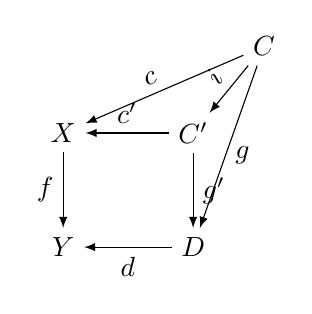
\begin{tikzpicture}[>=latex,baseline=(current bounding box.center),scale=1]
\node (X) at (0,0) {$X$};
\node (Y) at (0,-1.45) {$Y$};
\node (Cp) at (1.65,0) {$C'$};
\node (D) at (1.65,-1.45) {$D$};
\node (C) at (2.55,1.1) {$C$};
\draw[->] (C) -- node[above,sloped,pos=.55] {$c$} (X);
\draw[->] (C) -- node[above,sloped,pos=.50] {$i$} (Cp);
\draw[->] (C) -- node[right,pos=.55] {$g$} (D);
\draw[->] (Cp) -- node[above] {$c'$} (X);
\draw[->] (Cp) -- node[right] {$g'$} (D);
\draw[->] (X) -- node[left] {$f$} (Y);
\draw[->] (D) -- node[below] {$d$} (Y);
\end{tikzpicture}
\tag{3.7.2}
\end{equation}
对 $K\in\ob\Dctf(X)$，有典范箭头
\begin{equation}
f_*c_!c^!K\longrightarrow d_*d^!f_*K,
\tag{3.7.3}
\end{equation}
它是由伴随箭头 $i_*i^!\to\Id$ 定义的箭头
\[
f_*c_!c^!K=f_*c'_*(i_*i^!)c'^!K\longrightarrow f_*c'_*c'^!K=d_*g'_*c'^!K
\]
与同构
\[
d_*g'_*c'^!K\xrightarrow{\sim}d_*d^!f_*K
\]
的复合，后者由典范同构 $g'_*d'^!\xrightarrow{\sim}d^!f_*$（SGA 4 XVIII 3.1.12.3）定义。取 $K=\RHom_S(L_1,L_2)$，并将 3.7.3 与由 3.3.1 导出的同构复合，得到典范箭头
\begin{equation}
f_*c_*c^!\RHom_S(L_1,L_2)
\longrightarrow
 d_*d^!\RHom_S(f_{1!}L_1,f_{2*}L_2),
\tag{3.7.4}
\end{equation}
利用 3.2.1，可将它改写为
\begin{equation}
f_*c_!\RHom(c_1^*L_1,c_2^!L_2)
\longrightarrow
 d_*\RHom(d_1^*(f_{1!}L_1),d_2^!(f_{2*}L_2)).
\tag{3.7.5}
\end{equation}
于是得到
\begin{equation}
f_*:\Hom(c_1^*L_1,c_2^!L_2)
\longrightarrow
\Hom(d_1^*(f_{1!}L_1),d_2^!(f_{2*}L_2)).
\tag{3.7.6}
\end{equation}
箭头 3.7.5（相应地 3.7.6）推广了 3.3.1（相应地 3.3.2）；当 $c$、$d$ 是恒等态射时，两者相同。还须指出，当 $c$ 固有而 $f_1$、$f_2$、$d$ 为恒等箭头时，3.2.2（相应地 3.2.3）恰好就是 3.7.5（相应地 3.7.6）。当 $Y_1=Y_2=S=D$ 时，仍如上将 $f_*u$ 简记为 $u_*$。

\section{对应的配对。Lefschetz 公式}

\subsection*{4.1}
对 $i=1,2$，设 $X_i$ 是 $S$-概形，$X=X_1\times_SX_2$，$p_i:X\to X_i$ 是投影，$L_i\in\ob\Dctf(X_i)$，$K_{X_i}$ 是对偶化复形（1.3）。由 2.1.1 与求值箭头 2.2.2 复合而得的典范箭头
\begin{equation}
p_i^*\RHom(L_i,K_{X_i})\overset{\mathbf L}{\otimes}p_i^*L_i
\longrightarrow p_i^*K_{X_i},
\tag{4.1.1}
\end{equation}
在 $X$ 上取张量积，再与 Künneth 同构 1.7.6 复合，给出配对
\begin{equation}
(DL_1\overset{\mathbf L}{\otimes}_S L_2)\overset{\mathbf L}{\otimes}(L_1\overset{\mathbf L}{\otimes}_S DL_2)
\longrightarrow K_X,
\tag{4.1.2}
\end{equation}
利用 3.1.1 和 3.1.2，可改写为
\begin{equation}
\RHom_S(L_1,L_2)\overset{\mathbf L}{\otimes}\RHom_S(L_2,L_1)
\longrightarrow K_X.
\tag{4.1.3}
\end{equation}
由此导出一个称为杯积的配对
\begin{equation}
\langle\ ,\ \rangle:\Hom_S(L_1,L_2)\otimes\Hom_S(L_2,L_1)
\longrightarrow \H^0(X,K_X).
\tag{4.1.4}
\end{equation}
也可将 4.1.2 看作求值箭头
\[
DL_i\overset{\mathbf L}{\otimes}L_i\longrightarrow K_{X_i}.
\]
的外张量积。由 Künneth 同构 2.2.4 可知，4.1.2 是“完美对偶”，即通过伴随同构 2.2.1，将复形 $DL_1\overset{\mathbf L}{\otimes}_S L_2$、$L_1\overset{\mathbf L}{\otimes}_S DL_2$ 各自与另一个复形的对偶（取值于 $K_X$）认同。

当 $X_1=X_2=S$ 时，4.1.3 是任意赋环拓扑斯上完美复形的配对（SGA 6 I 7.8）的一个特例；采用（SGA 6 I 8.3）的记号，有
\begin{equation}
\langle u,v\rangle=\mathrm{Tr}(vu)=\mathrm{Tr}(uv).
\tag{4.1.5}
\end{equation}

\subsection*{4.2}
设 $c:C\to X$、$d:D\to X$，且 $e=c\times_Xd:E=C\times_XD\to X$。对 $P,Q\in\ob\Dctf(X)$，有典范箭头（通常不是同构）
\begin{equation}
c^!P\overset{\mathbf L}{\otimes}_X d^!Q
\longrightarrow e^!(P\overset{\mathbf L}{\otimes}Q),
\tag{4.2.1}
\end{equation}
与 1.7.3 一样，将它定义为下列复合箭头的伴随箭头
\[
e_!(c^!P\overset{\mathbf L}{\otimes}_X d^!Q)
\xrightarrow[(1)]{\sim}
 c_!c^!P\overset{\mathbf L}{\otimes}d_!d^!Q
\xrightarrow{(2)} P\overset{\mathbf L}{\otimes}Q,
\]
其中 (1) 是 Künneth 同构（SGA 4 XVII 5.4.2.2），(2) 是伴随箭头的张量积。对 4.2.1 应用 $e_!$，并与刚才引用的 Künneth 同构复合，得到典范箭头
\begin{equation}
c_!c^!P\overset{\mathbf L}{\otimes}d_!d^!Q
\longrightarrow e_!e^!(P\overset{\mathbf L}{\otimes}Q).
\tag{4.2.2}
\end{equation}
类似地，将 Künneth 箭头
\[
c_*c^!P\overset{\mathbf L}{\otimes}d_*d^!Q
\longrightarrow e_*(c^!P\overset{\mathbf L}{\otimes}_X d^!Q)
\]
与对 4.2.1 应用 $e_*$ 得到的箭头复合，得到典范箭头
\begin{equation}
c_*c^!P\overset{\mathbf L}{\otimes}d_*d^!Q
\longrightarrow e_*e^!(P\overset{\mathbf L}{\otimes}Q).
\tag{4.2.3}
\end{equation}
对于 $P=DL_1\overset{\mathbf L}{\otimes}_S L_2$、$Q=L_1\overset{\mathbf L}{\otimes}_S DL_2$，由 4.2.2 和 4.2.3，与 4.1.2 及同构 $e^!K_X=K_E$ 复合，再作 3.1.1 和 3.2.1 的认同，得到配对
\begin{equation}
c_!\RHom(c_1^*L_1,c_2^!L_2)\overset{\mathbf L}{\otimes}
 d_!\RHom(d_2^*L_2,d_1^!L_1)
\longrightarrow e_!K_E,
\tag{4.2.4}
\end{equation}
\begin{equation}
c_*\RHom(c_1^*L_1,c_2^!L_2)\overset{\mathbf L}{\otimes}
 d_*\RHom(d_2^*L_2,d_1^!L_1)
\longrightarrow e_*K_E,
\tag{4.2.4'}
\end{equation}
\begin{equation}
\langle\ ,\ \rangle:
\Hom(c_1^*L_1,c_2^!L_2)\otimes\Hom(d_2^*L_2,d_1^!L_1)
\longrightarrow \H^0(E,K_E).
\tag{4.2.5}
\end{equation}
这些配对与平展局部化相容：给定交换方块（未必为笛卡儿方块）
\[
\begin{tikzcd}[column sep=2.5em,row sep=1.5em]
& E' \arrow[dl] \arrow[dr] & && & E \arrow[dl] \arrow[dr] & \\
C' \arrow[dr] && D' \arrow[dl] & \text{在右图上平展} & C \arrow[dr] && D \arrow[dl] \\
& X &&&& X &
\end{tikzcd}
\]
若 $c'$、$d'$、$e'$ 表示复合 $C'\to C\to X$、$D'\to D\to X$、$E'\to E\to X$，则有交换方块


\begin{equation}
\tag{4.2.6}
\begin{tikzcd}[column sep=large,row sep=large]
\Hom(c_1^*L_1,c_2^!L_2)\otimes\Hom(d_2^*L_2,d_1^!L_1)
  \arrow[r,"4.2.5"] \arrow[d] &
\H^0(E,K_E)\arrow[d] \\
\Hom(c_1'{}^*L_1,c_2'{}^!L_2)\otimes\Hom(d_2'{}^*L_2,d_1'{}^!L_1)
  \arrow[r] &
\H^0(E',K_{E'})
\end{tikzcd}
\end{equation}
其中竖直箭头是限制，下面的水平箭头是类似于 4.2.5 的箭头与限制
\[
\H^0(E'',K_{E''})\longrightarrow \H^0(E',K_{E'}),
\]
的复合，这里 $E''=C'\times_{X'}D'$（对 4.2.4、4.2.4' 型箭头也有类似交换方块，留给读者写出）。若 $Z$ 在 $E$ 上平展，对于
\[
u\in\Hom(c_1^*L_1,c_2^!L_2),\qquad
v\in\Hom(d_2^*L_2,d_1^!L_1),
\]
\begin{equation}
\tag{4.2.7}
\langle u,v\rangle_Z\in \H^0(Z,K_Z)
\end{equation}
用此式表示 $\langle u,v\rangle$ 经限制在 $\H^0(Z,K_Z)$ 中的像（实际中 $Z$ 将是 $E$ 的一个连通分支）。若 $z$ 是 $E$ 的孤立闭点，$\bar z$ 是 $z$ 上方的几何点，则由 4.2.6 可知
\[
\langle u,v\rangle_z\in \H^0(z,K_z)=A
\]
只依赖于在 $\bar z$ 于 $C,D,X$ 中的像处作严格局部化所得的情形。

\begin{statement}{例 4.3}
设 $X_i$ 光滑且纯相对维数为 $r_i$，$c$、$d$ 是闭浸入，$c_2$（相应地 $d_1$）有限。当 $L_1=A_{X_1}$、$L_2=A_{X_2}$ 时，由 3.1.3 有
\[
DL_1\otimes_S^{\mathbf L}L_2=A_X(r_1)[2r_1],\qquad
L_1\otimes_S^{\mathbf L}DL_2=A_X(r_2)[2r_2],
\]
而 4.1.2 与乘积
\[
A_X(r_1)[2r_1]\otimes^{\mathbf L}A_X(r_2)[2r_2]\longrightarrow A_X(r)[2r],
\]
认同，其中 $r=r_1+r_2$；因此，考虑到 3.2.1，4.2.5 与通常的杯积
\[
\H_C^{2r_1}(X,A(r_1))\otimes \H_D^{2r_2}(X,A(r_2))
\longrightarrow
\H_{C\cap D}^{2r}(X,A(r)).
\]
认同。取 $c$（相应地 $d$）的类为从 $X_1$ 到 $X_2$（相应地从 $X_2$ 到 $X_1$）的上同调对应（3.2 a)）。由（SGA $4^{1/2}$，圈 2.3.8）可知，在 $C\cap D$ 的孤立点 $z$ 处，$\langle \cl(c),\cl(d)\rangle_z$ 就是 $C$ 与 $D$ 在 $z$ 处的相交重数在 $A$ 中的像。
\end{statement}

现在给出本报告的主要结果。

\begin{statement}{定理 4.4}
对 $i=1,2$，设 $f_i:X_i\longrightarrow Y_i$ 是固有 $S$-态射，
\[
f=f_1\times_S f_2:X\longrightarrow Y,\qquad
p_i:X\longrightarrow X_i,\qquad q_i:Y\longrightarrow Y_i
\]
为投影。再设
\begin{equation}
\tag{4.4.0}
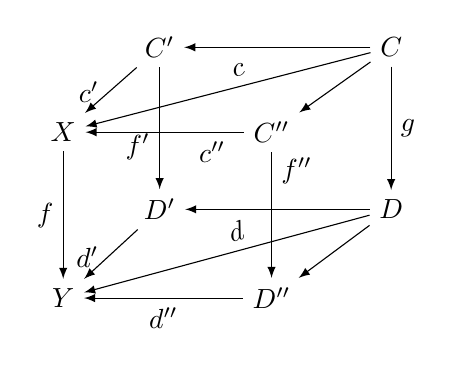
\begin{tikzpicture}[>=latex,baseline=(current bounding box.center),scale=0.98]
\node (Cp) at (0,2.1) {$C'$};
\node (C) at (3.0,2.1) {$C$};
\node (X) at (-1.25,1.0) {$X$};
\node (Cpp) at (1.45,1.0) {$C''$};
\node (Dp) at (0,0) {$D'$};
\node (D) at (3.0,0) {$D$};
\node (Y) at (-1.25,-1.15) {$Y$};
\node (Dpp) at (1.45,-1.15) {$D''$};
\draw[->] (C) -- (Cp);
\draw[->] (Cp) -- node[left,pos=.55] {$c'$} (X);
\draw[->] (C) -- node[above,sloped,pos=.45] {$c$} (X);
\draw[->] (C) -- (Cpp);
\draw[->] (Cpp) -- node[below,pos=.20] {$c''$} (X);
\draw[->] (Cp) -- node[left,pos=.65] {$f'$} (Dp);
\draw[->] (Cpp) -- node[right,pos=.15] {$f''$} (Dpp);
\draw[->] (C) -- node[right] {$g$} (D);
\draw[->] (X) -- node[left] {$f$} (Y);
\draw[->] (D) -- (Dp);
\draw[->] (Dp) -- node[left,pos=.55] {$d'$} (Y);
\draw[->] (D) -- node[above,sloped,pos=.45] {$d$} (Y);
\draw[->] (D) -- (Dpp);
\draw[->] (Dpp) -- node[below] {$d''$} (Y);
\end{tikzpicture}
\end{equation}
是水平面为笛卡儿方块的交换立方图，其中 $c'$、$c''$、$d'$、$d''$ 固有。令
\[
c_i'=p_i c',\qquad c_i''=p_i c'',\qquad d_i'=q_i d',\qquad d_i''=q_i d''.
\]
最后，设 $L_i\in\ob \Dctf(X_i)$。则有交换方块
\begin{equation}
\tag{4.4.1}
\begin{tikzcd}[column sep=huge,row sep=huge]
f_*c'_*\RHom(c_1'{}^*L_1,c_2'{}^!L_2)\otimes^{\mathbf L}
f_*c''_*\RHom(c_2''{}^*L_2,c_1''{}^!L_1)
 \arrow[r,"(1)"] \arrow[d,"(2)"'] &
f_*c_*K_C \arrow[d,"(4)"] \\
d'_*\RHom(d_1'{}^*M_1,d_2'{}^!M_2)\otimes^{\mathbf L}
d''_*\RHom(d_2''{}^*M_2,d_1''{}^!M_1)
 \arrow[r,"(3)"'] &
d_*K_D ,
\end{tikzcd}
\end{equation}
其中 $M_i=f_{i*}L_i$，$(3)$ 由 4.2.4 给出，$(1)$ 由 4.2.4 应用 $f_*$ 并与典范箭头
\[
f_*c'_*(-)\otimes^{\mathbf L} f_*c''_*(-)\longrightarrow f_*(c'_*(-)\otimes^{\mathbf L}c''_*(-)),
\]
复合而得，$(2)$ 是关于包含 $f$ 的两个面的箭头 3.7.5 的张量积，$(4)$ 则由伴随箭头 $g_*K_C=g_!g^!K_D\longrightarrow K_D$ 定义。
\end{statement}

\begin{prooftext}[证明]
令
\[
DL_1\otimes_S^{\mathbf L}L_2=P,\qquad
L_1\otimes_S^{\mathbf L}DL_2=Q,\qquad
DM_1\otimes_S^{\mathbf L}M_2=E,\qquad
M_1\otimes_S^{\mathbf L}DM_2=F.
\]
考虑图
\begin{equation}
\tag{4.4.2}
{
\begin{tikzcd}[column sep=2.6em,row sep=2.6em]
f_*c'_*c'{}^!P\otimes^{\mathbf L} f_*c''_*c''{}^!Q
  \arrow[rr,"(1)"] \arrow[d,"(8)"'] &&
f_*c_*c^!\bigl(P\otimes^{\mathbf L}Q\bigr)
  \arrow[r,"(2)"] \arrow[d,"(9)"'] &
f_*c_*c^!K_X \arrow[d,"(10)"]\\
d'_*d'{}^!f_*P\otimes^{\mathbf L}d''_*d''{}^!f_*Q
  \arrow[r,"(3)"'] \arrow[d,"(11)"'] &
d_*d^!\bigl(f_*P\otimes^{\mathbf L}f_*Q\bigr)
  \arrow[r,"(4)"'] \arrow[d,"(12)"'] &
d_*d^!f_*\bigl(P\otimes^{\mathbf L}Q\bigr)
  \arrow[r,"(5)"'] &
d_*d^!f_*K_X \arrow[d,"(13)"]\\
d'_*d'{}^!E\otimes^{\mathbf L}d''_*d''{}^!F
  \arrow[r,"(6)"'] &
d_*d^!\bigl(E\otimes^{\mathbf L}F\bigr)
  \arrow[rr,"(7)"'] &&
d_*d^!K_Y,
\arrow[from=1-1,to=2-2, phantom, "\scriptstyle (A)"]
\arrow[from=1-3,to=2-4, phantom, "\scriptstyle (B)"]
\arrow[from=2-1,to=3-2, phantom, "\scriptstyle (C)"]
\arrow[from=2-2,to=3-4, phantom, "\scriptstyle (D)"]
\end{tikzcd}
}
\end{equation}
各箭头如下：$(1)$ 由 4.2.2 应用 $f_*$ 而得；$(2)$ 由 4.1.2 定义；$(3)$ 由 4.2.2 给出；$(4)$ 由典范箭头 $f_*P\otimes^{\mathbf L}f_*Q\longrightarrow f_*(P\otimes^{\mathbf L}Q)$ 给出；$(5)$ 由 4.1.2 给出；$(6)$ 由 4.2.2 给出；$(7)$ 由 4.1.2 给出；$(8)$ 是箭头 3.7.3 的张量积；$(9)$、$(10)$ 由 3.7.3 定义；$(11)$、$(12)$ 由同构 $f_*P\longrightarrow E$、$f_*Q\longrightarrow F$（3.3.1）定义；$(13)$ 由伴随箭头 $f_*K_X\longrightarrow K_Y$ 定义。按定义，经 3.1.1 和 3.2.1 认同后，4.4.1 就是 4.4.2 的外边界。只需证明方块 $(A)$、$(B)$、$(C)$、$(D)$ 交换。由函子性，$(B)$、$(C)$ 的交换性显然。剩下要证明 $(A)$、$(D)$ 的交换性。

a) $(D)$ 的交换性。只需证明方块
\begin{equation}
\tag{4.4.3}
\begin{tikzcd}[column sep=large,row sep=large]
f_*P\otimes^{\mathbf L}f_*Q \arrow[r] \arrow[d] & f_*K_X \arrow[d]\\
E\otimes^{\mathbf L}F \arrow[r] & K_Y
\end{tikzcd}
\end{equation}
（即 $d=\Id$ 时的 $(D)$）交换。回顾配对
\[
P\otimes^{\mathbf L}Q\longrightarrow K_X
\quad(\text{相应地 }E\otimes^{\mathbf L}F\longrightarrow K_Y)
\]
是求值箭头
\[
DL_i\otimes^{\mathbf L}L_i\longrightarrow K_{X_i}
\quad(\text{相应地 }DM_i\otimes^{\mathbf L}M_i\longrightarrow K_{Y_i}).
\]
的外张量积。由 Künneth 同构
\[
f_{1*}DL_1\otimes_S^{\mathbf L} f_{2*}L_2 \lisom f_*P,\qquad
f_{1*}L_1\otimes_S^{\mathbf L} f_{2*}DL_2 \lisom f_*Q,
\]
可将 4.4.3 与下列方块的外张量积认同
\begin{equation}
\tag{4.4.4}
\begin{tikzcd}[column sep=large,row sep=large]
f_{i*}DL_i\otimes^{\mathbf L} f_{i*}L_i
 \arrow[r,"(1)"] \arrow[d,"(3)"'] &
f_{i*}K_{X_i} \arrow[d,"(4)"]\\
DM_i\otimes^{\mathbf L}M_i \arrow[r,"(2)"'] & K_{Y_i},
\end{tikzcd}
\end{equation}
其中 $(2)$ 是求值箭头，$(1)$ 是典范箭头
\[
f_{i*}DL_i\otimes^{\mathbf L} f_{i*}L_i\longrightarrow f_{i*}(DL_i\otimes^{\mathbf L}L_i)
\]
与由求值箭头定义的箭头的复合，$(3)$ 是对偶同构 $f_{i*}DL_i\longrightarrow DM_i$ 与 $M_i$ 的恒等箭头的张量积，$(4)$ 是伴随箭头。因此只需验证方块 4.4.4 交换。由于上述对偶同构是典范箭头（SGA 4 XVIII 3.1.9.5）
\[
f_{i*}\RHom(L_i,K_{X_i})\longrightarrow \RHom(f_{i*}L_i,f_{i*}K_{X_i})
\]
与由伴随箭头
\[
f_{i*}K_{X_i}\longrightarrow K_{Y_i},
\]
导出的箭头的复合，故只需说明下列方块交换：
\begin{equation}
\tag{4.4.5}
\begin{tikzcd}[column sep=large,row sep=large]
f_{i*}\RHom(L_i,K_{X_i})\otimes^{\mathbf L} f_{i*}L_i
 \arrow[r,"(1)"] \arrow[d,"(3)"'] &
f_{i*}K_{X_i} \arrow[d,"\Id"]\\
\RHom(f_{i*}L_i,f_{i*}K_{X_i})\otimes^{\mathbf L} f_{i*}L_i
 \arrow[r,"(2)"'] &
f_{i*}K_{X_i},
\end{tikzcd}
\end{equation}
其中 $(1)$ 是 4.4.4 的箭头 $(1)$，$(2)$ 是求值箭头，$(3)$ 是刚才所述典范箭头与 $f_{i*}L_i$ 的张量积。更一般地，对于 $\Dctf(X_i)$ 中的任意箭头 $N_i\longrightarrow f_{i*}L_i$，即位于 $f_i$ 上的任意 $1$ 型箭头 $L_i\xrightarrow{u}N_i$，由 4.4.5 导出的三角形
\[
\begin{tikzcd}[column sep=large,row sep=large]
f_{i*}\RHom(L_i,K_{X_i})\otimes^{\mathbf L}N_i
 \arrow[dr] \arrow[d] & \\
\RHom(N_i,f_{i*}K_{X_i})\otimes^{\mathbf L}N_i \arrow[r] &
f_{i*}K_{X_i}
\end{tikzcd}
\]
交换：事实上，由函子性，可设 $L_i=f_i^*N_i$，且 $u$ 由 $L_i$ 的恒等态射给出；此时箭头
\[
f_{i*}\RHom(L_i,K_{X_i})\longrightarrow\RHom(N_i,f_{i*}K_{X_i})
\]
是平凡对偶同构的逆，取 $N_i$ 的平坦预解和 $K_{X_i}$ 的内射预解，便可直接在复形层面验证该三角形交换。

b) $(A)$ 的交换性。查阅 3.7.3 的定义，可知只需在下列每种情形验证此交换性：
\[
\text{(i) } X_i=Y_i,\quad f_i=\text{恒等箭头，定义于 }X_i;\qquad
\text{(ii) 4.4.0 的各侧面为笛卡儿方块。}
\]
先考虑情形 (i)。方块 $(A)$ 是下图的外边界
\[
\begin{tikzcd}[column sep=large,row sep=large]
c'_*c'{}^!P\otimes^{\mathbf L}c''_*c''{}^!Q
 \arrow[r,"\sim"] \arrow[d,"(8)"'] &
c_*\bigl(c'{}^!P\otimes_X^{\mathbf L}c''{}^!Q\bigr)
 \arrow[r] \arrow[d] &
c_*c^!(P\otimes^{\mathbf L}Q)\arrow[d,"(9)"]\\
d'_*d'{}^!P\otimes^{\mathbf L}d''_*d''{}^!Q
 \arrow[r,"\sim"'] &
d_*\bigl(d'{}^!P\otimes_X^{\mathbf L}d''{}^!Q\bigr)
 \arrow[r] &
d_*d^!(P\otimes Q),
\arrow[from=1-1,to=2-2,phantom,"\scriptstyle A_1"]
\arrow[from=1-2,to=2-3,phantom,"\scriptstyle A_2"]
\end{tikzcd}
\]
其中 $A_1$ 的水平同构为 Künneth 同构，$A_2$ 的水平箭头由 4.2.1 给出，中间的竖直箭头则由下列箭头应用 $d_*$ 而得
\[
g_!(c'{}^!P\otimes_X^{\mathbf L}c''{}^!Q)\longrightarrow d'{}^!P\otimes_X^{\mathbf L}d''{}^!Q
\]
该箭头通过 Künneth 同构由伴随箭头
\[
f'_!c'{}^!P\longrightarrow d'{}^!P,\qquad
f''_!c''{}^!Q\longrightarrow d''{}^!Q.
\]
的外张量积定义。这些伴随箭头与 $d'_!d'{}^!P$、$d''_!d''{}^!Q$ 的恒等箭头给出位于
\[
\begin{tikzcd}[column sep=large,row sep=large]
& c'{}^!P \arrow[d] \arrow[dl] & & c''{}^!Q \arrow[d]\arrow[dl]\\
d'_!d'{}^!P & d'{}^!P\arrow[l] & d''_!d''{}^!Q & d''{}^!Q\arrow[l]
\end{tikzcd}
\]
下列图上的 $3$ 型箭头的交换三角形（1.4）：
\[
\begin{tikzcd}[column sep=large,row sep=large]
& C' \arrow[d,"f'"] \arrow[dl,"c'"']\\
X & D'\arrow[l,"d'"]
\end{tikzcd}
\qquad
\begin{tikzcd}[column sep=large,row sep=large]
& C'' \arrow[d,"f''"] \arrow[dl,"c''"']\\
X & D''\arrow[l,"d''"]
\end{tikzcd}.
\]
通过（在 $X$ 上）取外张量积，这些三角形给出交换三角形
\[
\begin{tikzcd}[column sep=huge,row sep=large]
& c'{}^!P\otimes_X^{\mathbf L}c''{}^!Q \arrow[d] \arrow[dl]\\
d'_!d'{}^!P\otimes d''_!d''{}^!Q &
d'{}^!P\otimes_X^{\mathbf L}d''{}^!Q\arrow[l]
\end{tikzcd}
\qquad\text{位于下图上}\qquad
\begin{tikzcd}[column sep=large,row sep=large]
& C\arrow[d,"g"]\arrow[dl,"c"']\\
X & D\arrow[l,"d"]
\end{tikzcd}.
\]
此三角形的交换性等价于将 $A_1$ 的水平箭头取逆所得方块的交换性。另一方面，有由 $d'{}^!P$、$c'{}^!P$、$d''{}^!Q$、$c''{}^!Q$ 的恒等箭头定义的 $3$ 型箭头的交换三角形
\[
\begin{tikzcd}[column sep=large,row sep=large]
& c'{}^!P \arrow[d]\arrow[dl]\\
P & d'{}^!P\arrow[l]
\end{tikzcd}
\qquad
\begin{tikzcd}[column sep=large,row sep=large]
& c''{}^!Q \arrow[d]\arrow[dl]\\
Q & d''{}^!Q\arrow[l]
\end{tikzcd}
\]
。取外张量积后，得到交换三角形
\[
\begin{tikzcd}[column sep=huge,row sep=large]
& c'{}^!P\otimes_X^{\mathbf L}c''{}^!Q \arrow[d]\arrow[dl]\\
P\otimes^{\mathbf L}Q & d'{}^!P\otimes_X^{\mathbf L}d''{}^!Q\arrow[l]
\end{tikzcd}
\]
可将它解释为位于 $g:C\longrightarrow D$ 上的 $3$ 型箭头之间的态射：
\[
\begin{tikzcd}[column sep=large,row sep=large]
c'{}^!P\otimes_X^{\mathbf L}c''{}^!Q \arrow[r]\arrow[d] &
c'{}^!(P\otimes^{\mathbf L}Q)\arrow[d]\\
d'{}^!P\otimes_X^{\mathbf L}d''{}^!Q \arrow[r] &
d'{}^!(P\otimes Q),
\end{tikzcd}
\]
也可解释为 $D$ 上的交换方块：
\[
\begin{tikzcd}[column sep=large,row sep=large]
g_*(c'{}^!P\otimes_X^{\mathbf L}c''{}^!Q) \arrow[r]\arrow[d] &
g_*c'{}^!(P\otimes^{\mathbf L}Q)\arrow[d]\\
d'{}^!P\otimes_X^{\mathbf L}d''{}^!Q \arrow[r] &
d^!(P\otimes^{\mathbf L}Q).
\end{tikzcd}
\]
但对后一个方块应用 $d_*$，所得恰是 $A_2$，从而得到情形 (i) 中 $(A)$ 的交换性。

剩下处理情形 (ii)。由于 4.4.0 中包含 $f$ 的两个面是笛卡儿方块，箭头
\[
f'_*c'{}^!P\longrightarrow d'{}^!f_*P,\qquad
f''_*c''{}^!Q\longrightarrow d''{}^!f_*Q
\]
（3.7.3）是同构。它们的逆在 $f'$、$f''$ 上定义 $1$ 型箭头
\[
c'{}^!P\longrightarrow d'{}^!f_*P,\qquad
c''{}^!Q\longrightarrow d''{}^!f_*Q
\]
，由此取正像，得到位于 4.4.0 中包含 $f$ 的两个面上的 $1$ 型箭头的交换方块
\[
\begin{tikzcd}[column sep=large,row sep=large]
c'_*c'{}^!P \arrow[d] & c'{}^!P\arrow[l]\arrow[d]\\
d'_*d'{}^!P & d'{}^!f_*P\arrow[l]
\end{tikzcd}
\qquad
\begin{tikzcd}[column sep=large,row sep=large]
c''_*c''{}^!Q \arrow[d] & c''{}^!Q\arrow[l]\arrow[d]\\
d''_*d''{}^!Q & d''{}^!f_*Q\arrow[l]
\end{tikzcd}
\]
。取张量积，得到 $\Dctf(Y)$ 中的交换方块
\begin{equation}
\tag{4.4.6}
{
\begin{tikzcd}[column sep=large,row sep=large]
d'_*d'{}^!f_*P\otimes^{\mathbf L}d''_*d''{}^!f_*Q
 \arrow[r]\arrow[d] &
d_*\bigl(d'{}^!f_*P\otimes_Y^{\mathbf L}d''{}^!f_*Q\bigr)\arrow[d]\\
f_*c'_*c'{}^!P\otimes^{\mathbf L}f_*c''_*c''{}^!Q
 \arrow[r] &
d_*g_*\bigl(c'{}^!P\otimes_X^{\mathbf L}c''{}^!Q\bigr),
\end{tikzcd}
}
\end{equation}
其中左侧竖直箭头是 $(8)$ 的逆，水平箭头由 Künneth 同构给出，右侧竖直箭头由下列箭头在 $Y$ 上的外张量积给出
\[
f'_*c'{}^!P\longrightarrow d'{}^!f_*P,\qquad
f''_*c''{}^!Q\longrightarrow d''{}^!f_*Q.
\]
同一张量积定义了方块
\begin{equation}
\tag{4.4.7}
\begin{tikzcd}[column sep=large,row sep=large]
d'{}^!f_*P\otimes_Y^{\mathbf L}d''{}^!f_*Q
 \arrow[r]\arrow[d] &
d^!f_*(P\otimes^{\mathbf L}Q)\arrow[d]\\
g_*(c'{}^!P\otimes_X^{\mathbf L}c''{}^!Q)
 \arrow[r] &
g_*c'{}^!(P\otimes^{\mathbf L}Q),
\end{tikzcd}
\end{equation}
左侧的竖直箭头，其中右侧竖直箭头为 3.7.3，水平箭头由 4.2.1 定义。将 4.4.6 与 $d_*(4.4.7)$ 合成的图，其外边界就是将 $(A)$ 的竖直箭头取逆所得的方块。因此只需证明 4.4.7 交换，换言之，即证明箭头 4.2.1
\[
c'{}^!P\otimes_X^{\mathbf L}c''{}^!Q\longrightarrow c'{}^!(P\otimes^{\mathbf L}Q),\qquad
d'{}^!f_*P\otimes_Y^{\mathbf L}d''{}^!f_*Q\longrightarrow d^!f_*(P\otimes^{\mathbf L}Q)
\]
在被视为位于 $g$ 上的 $1$ 型箭头时，定义了从
\[
c'{}^!P\otimes_X^{\mathbf L}c''{}^!Q\longrightarrow d'{}^!f_*P\otimes_Y^{\mathbf L}d''{}^!f_*Q
\]
到
\[
c'{}^!(P\otimes^{\mathbf L}Q)\longrightarrow d^!f_*(P\otimes^{\mathbf L}Q),
\]
的态射。由伴随，只需验证伴随箭头的张量积
\[
c'_*c'{}^!P\otimes_X^{\mathbf L}c''_*c''{}^!Q\longrightarrow P\otimes^{\mathbf L}Q,
\qquad
d'_*d'{}^!f_*P\otimes_Y^{\mathbf L}d''_*d''{}^!f_*Q
\longrightarrow f_*P\otimes^{\mathbf L}f_*Q
\]
在位于 $f$ 上的 $1$ 型箭头之间，定义从下列箭头的张量积
\[
c'_*c'{}^!P\longrightarrow d'_*d'{}^!f_*P,\qquad
c''_*c''{}^!Q\longrightarrow d''_*d''{}^!f_*Q
\]
到下列箭头的张量积的态射
\[
P\longrightarrow f_*P,\qquad Q\longrightarrow f_*Q.
\]
为此，只需验证伴随箭头
\[
c'_*c'{}^!P\longrightarrow P,\qquad d'_*d'{}^!f_*P\longrightarrow f_*P
\]
定义了从
\[
c'_*c'{}^!P\longrightarrow d'_*d'{}^!f_*P
\]
到
\[
P\longrightarrow f_*P,
\]
的态射，对 $(c'',d'')$ 也同样成立。两种情形陈述相同，故只需考虑 $(c',d')$。须说明三角形
\[
\begin{tikzcd}[column sep=large,row sep=large]
& f_*c'_*c'{}^!P \arrow[d,"\sim"]\arrow[dl]\\
f_*P & d'_*d'{}^!f_*P\arrow[l]
\end{tikzcd}
\]
交换，其中水平和斜箭头由伴随给出，竖直箭头由同构 3.7.3 给出。考虑到 3.7.3 的定义（SGA 4 XVIII 3.1.12.3），它是基变换同构的转置，故应用函子 $\Hom(R,-)$（$R\in\ob\Dctf(Y)$）后，只需验证下列方块的交换性
\[
\begin{tikzcd}[column sep=large,row sep=large]
c'_*c'{}^*f^*R \arrow[r,"\Id"] &
c'_*f'{}^*d'{}^*R\\
f^*R \arrow[u] \arrow[r] &
f^*d'_*d'{}^*R\arrow[u,"\sim"']
\end{tikzcd}
\]
其中左侧竖直箭头（相应地下面的水平箭头）由伴随箭头 $1\longrightarrow c'_*c'{}^*$（相应地 $1\longrightarrow d'_*d'{}^*$）定义，右侧竖直箭头由基变换同构
\[
f^*d'_*\lisom c'_*f'{}^*.
\]
定义。但此方块由基变换箭头的定义即知交换。由此证明 $(A)$ 的交换性，也完成了定理的证明。
\end{prooftext}

\begin{statement}{推论 4.5}
在 4.4 的假设下，有交换方块
\[
\begin{tikzcd}[column sep=large,row sep=large]
\Hom(c_1'{}^*L_1,c_2'{}^!L_2)\otimes
\Hom(c_2''{}^*L_2,c_1''{}^!L_1)
 \arrow[r,"4.2.5"] \arrow[d,"3.7.6\otimes 3.7.6"'] &
\H^0(C,K_C)\arrow[d,"g_*"]\\
\Hom(d_1'{}^*f_{1*}L_1,d_2'{}^!f_{2*}L_2)\otimes
\Hom(d_2''{}^*f_{2*}L_2,d_1''{}^!f_{1*}L_1)
 \arrow[r,"4.2.5"'] &
\H^0(D,K_D),
\end{tikzcd}
\]
其中 $g_*$ 由伴随箭头
\[
g_*K_C=g_*g^!K_D\longrightarrow K_D.
\]
定义。换言之，对于
\[
u\in\Hom(c_1'{}^*L_1,c_2'{}^!L_2),\qquad
v\in\Hom(c_2''{}^*L_2,c_1''{}^!L_1),
\]
有
\begin{equation}
\tag{4.5.1}
\langle f_*u,f_*v\rangle=g_*\langle u,v\rangle.
\end{equation}
\end{statement}

对于每个固有 $S$-概形 $t:T\longrightarrow S$，用
\begin{equation}
\tag{4.6}
\int_T:\H^0(T,K_T)\longrightarrow \H^0(S,K_S)=\H^0(S,A)
\end{equation}
表示由下列伴随箭头定义的箭头
\[
t_!K_T\longrightarrow A.
\]

\begin{statement}{推论 4.7 --- Lefschetz--Verdier 公式}
在 4.4 的假设下，设 $Y_1=Y_2=S=D'=D''$。对于
\[
u\in\Hom(c_1'{}^*L_1,c_2'{}^!L_2),\qquad
v\in\Hom(c_2''{}^*L_2,c_1''{}^!L_1),
\]
有
\begin{equation}
\tag{4.7.1}
\langle u_*,v_*\rangle=\int_C\langle u,v\rangle,
\end{equation}
其中
\[
u_*\in\Hom(f_{1*}L_1,f_{2*}L_2),\qquad
v_*\in\Hom(f_{2*}L_2,f_{1*}L_1)
\]
是由 $u$、$v$ 取 $S$ 上的正像导出的同态（3.7.6），而
\[
\langle u_*,v_*\rangle=\Tr(u_*v_*)=\Tr(v_*u_*)
\]
是完美复形同态 $u_*$、$v_*$ 在（SGA 6 I 8.3）意义下的杯积（4.1.5）。
\end{statement}

结合 3.6.5，特别得到：

\begin{statement}{推论 4.8}
设 $t:T\longrightarrow S$ 是固有 $S$-概形，$\Delta\subset T\times_S T$ 是对角线，$F:T\longrightarrow T$ 是 $T$ 的一个 $S$-自同态，$T^F=(\text{图像 }F)\times_{(T\times_S T)}\Delta$ 是 $F$ 的不动点概形，$L\in\ob\Dctf(T)$，$u\in\Hom(F^*L,L)$ 是从 $L$ 到 $L$、支集在 $F$ 的图像中的对应，$1\in\Hom(L,L)$ 是支集在 $\Delta$ 中的恒等对应（3.2 b)）。则
\[
\Tr(u_*)=\int_{T^F}\langle u,1\rangle,
\]
其中 $u_*$ 是将 $t_*L\longrightarrow t_*F^*L$（逆像）与 $t_*u:t_*F^*L\longrightarrow t_*L$ 复合所得的 $t_*L$ 的自同态。
\end{statement}

由 3.2 a) 和 3.6 的注记，还可推出：

\begin{statement}{推论 4.9}
在 4.7 的假设下，设 $X_i$ 在 $S$ 上光滑且纯相对维数为 $r_i$，$C'$（相应地 $C''$）是 $X$ 的闭子概形，在 $X_2$（相应地 $X_1$）上有限且具有有限 Tor 维数。设
\[
\cl(C')\in \H_{C'}^{2r_1}(X,A(r_1)),\qquad
\cl(C'')\in \H_{C''}^{2r_2}(X,A(r_2))
\]
分别为 $C'$、$C''$ 的上同调类，且设
\[
\cl(C')_*\in\Hom(\R f_{1*}A,\R f_{2*}A),\qquad
\cl(C'')_*\in\Hom(\R f_{2*}A,\R f_{1*}A)
\]
为对应的同态（3.2 a)、3.7.6）。则
\[
\langle \cl(C')_*,\cl(C'')_*\rangle
=
\int_{C'\cap C''}\cl(C)\cl(D),
\]
其中
\[
\cl(C)\cl(D)\in
\H_{C'\cap C''}^{2(r_1+r_2)}(X,A(r_1+r_2))
=
\H^0(C'\cap C'',K_{C'\cap C''})
\]
为通常的杯积。
\end{statement}

结合 4.3，特别得到：

\begin{statement}{推论 4.10}
在 4.9 的假设下，设 $C'\cap C''$ 有限。对 $z\in C'\cap C''$，用 $(C'\!\cdot C'')_z$ 表示 $C'$ 与 $C''$ 在 $z$ 处的相交重数在 $A$ 中的像。则
\[
\langle \cl(C')_*,\cl(C'')_*\rangle
=
\sum_{z\in C'\cap C''}(C'\!\cdot C'')_z.
\]
\end{statement}

\begin{statement}{4.11}
在 4.9 的假设下，一般有
\begin{equation}
\tag{4.11.1}
\langle \cl(C')_*,\cl(C'')_*\rangle
=
\sum_{Z\in\pi_0(C'\cap C'')}(\cl(C')\cl(C''))_Z,
\end{equation}
其中 $\pi_0(C'\cap C'')$ 表示 $C'\cap C''$ 的连通分支集合，$(\cl(C')\cl(C''))_Z$ 是 $\cl(C')\cl(C'')$ 在 $\H^0(Z,K_Z)$ 中的限制。当 $Z$ 是维数 $\geq 1$ 的分支时，计算 $(\cl(C')\cl(C''))_Z$ 会遇到困难，因为此时处于“超额”情形。若 $Z$ 光滑且纯维数为 $d$，$C'$、$C''$ 在 $Z$ 的一个邻域中光滑，并且 $X$ 射影，则可以证明
\begin{equation}
\tag{4.11.2}
\int_Z(\cl(C')\cl(C''))_Z=\int_Z c_d(N_Z),
\end{equation}
其中 $N_Z$ 是由法丛正合列
\[
0\longrightarrow N_{Z/C'}\oplus N_{Z/C''}\longrightarrow N_{Z/X}\longrightarrow N_Z\longrightarrow 0,
\]
定义的秩为 $d$ 的局部自由层，$c_d(N_Z)\in \H^{2d}(Z,A(d))$ 表示其第 $d$ 个 Chern 类（SGA 5 VII）（利用（SGA 6 XIV 6.3）归约到 K 理论中相交数的计算，再应用（SGA 6 VII 2.5），参见（[10] 4.1）；射影性假设大概可以去掉）。

设 $T$ 是光滑射影 $S$-概形；取 $S$-自同态 $F$ 的图像（相应地对角线）为对应 $C'$（相应地 $C''$），并设不动点概形 $T^F=C'\cap C''$ 光滑。上面的层 $N_{(T^F)}$ 就是 $T^F$ 的切层，因此，由 Gauss--Bonnet 公式（SGA 5 VII 4.9），4.11.2 蕴含与拓扑学中一个著名公式相对应的公式：
\begin{equation}
\tag{4.11.3}
\Tr(F,\R\Gamma(T,A))=\EP(T^F),
\end{equation}
其中 $\EP(T^F)$ 表示 $T_s^F$ 的 Euler--Poincaré 示性数，$s$ 是 $S$ 上方的一个几何点（见所引文献）。
\end{statement}

当 $Z$ 是非光滑且维数 $\geq 1$ 的分支时，如何计算 $(\cl(C')\cl(C''))_Z$，至少据整理者所知，一般情形尚未得到处理。

\begin{statement}{4.12}
在 4.7 的情形中，设 $z$ 是 $C$ 的孤立点，其在 $X_i$ 上的投影为 $z_i$，在 $C'$（相应地 $C''$）上的投影为 $a'$（相应地 $a''$）；又设 $\bar z$ 是 $z$ 上方的几何点，其在 $z_i$ 上方的像为 $\bar z_i$。假设 $c_2'$（相应地 $c_1''$）在 $a'$（相应地 $a''$）处拟有限且平坦，$L_i$ 在 $\bar z_i$ 的一个邻域中完美，并且 $u$（相应地 $v$）在 $a'$（相应地 $a''$）的一个邻域中由
\[
\Tr_{c_2'}:c_{2!}'c_2'{}^*L_2\longrightarrow L_2
\quad\text{且}\quad
s\in\Hom(c_1'{}^*L_1,c_2'{}^*L_2)
\]
给出（相应地由
\[
\Tr_{c_1''}:c_{1!}''c_1''{}^*L_1\longrightarrow L_1
\quad\text{且}\quad
t\in\Hom(c_2''{}^*L_2,c_1''{}^*L_1)).
\]
给出）。设 $s_{\bar z}\in\Hom(L_{1\bar z_1},L_{2\bar z_2})$（相应地 $t_{\bar z}\in\Hom(L_{2\bar z_2},L_{1\bar z_1})$）为由 $s$（相应地 $t$）取纤维得到的同态。再如 3.2 a)，用 $\cl(c')$（相应地 $\cl(c'')$）表示由 $c_2'$（相应地 $c_1''$）在 $a'$（相应地 $a''$）的一个邻域中定义的从 $X_1$ 到 $X_2$（相应地从 $X_2$ 到 $X_1$）的对应；用 $(C'\!\cdot C'')_z$ 表示相应局部项 $\langle\cl(c'),\cl(c'')\rangle_z$（当 $C'$、$C''$ 是 $X$ 的闭子概形且 $X_1$、$X_2$ 光滑时，它等于 $C'$、$C''$ 在 $z$ 处的相交重数在 $A$ 中的像）。则：
\begin{equation}
\tag{4.12.1}
\langle u,v\rangle_z=(C'\!\cdot C'')_z\langle s_{\bar z},t_{\bar z}\rangle.
\end{equation}
这很容易由 4.2.6 推出。
\end{statement}

\begin{statement}{4.13}
若 $T$ 是 $S$ 上的概形，用 $DF(T)$ 表示具有有限滤过的 $A_T$-模复形的滤过导出范畴（[9] V 1），用 $DF_{\ctf}(T)$ 表示由满足 $\gr(L)\in\ob\Dctf(T)$ 的 $L$ 组成的满子范畴。滤过导出函子与取相伴分次对象之间的相容性，保证 $DF_{\ctf}$ 在六种运算 $f^*$、$f_*$、$f_!$、$f^!$、$\otimes^{\mathbf L}$、$\RHom$ 下稳定。对前几节的定义和结果作必要修改后，它们在 $DF_{\ctf}$ 中仍然成立。配对 4.1.2 与取相伴分次对象相容（将 $K_X$ 看作带有平凡滤过），因此，采用 4.2.5 的记号，对 $L_i\in\ob DF_{\ctf}(X_i)$，
\[
u\in\Hom_{DF}(c_1^*L_1,c_2^!L_2),\qquad
v\in\Hom_{DF}(d_2^*L_2,d_1^!L_1),
\]
在 $\H^0(E,K_E)$ 中有下列等式：
\begin{equation}
\tag{4.13.1}
\langle u,v\rangle=\sum_i\langle \gr^i u,\gr^i v\rangle.
\end{equation}
正如 Deligne 所指出，这一观察特别适用于 Langlands 在（[13] 第~7 节）考虑的情形。他在所引文献 7.11 中考虑的对应，在不动点附近确实保持层上的有限滤过，其相伴分次对象在不动点的像处作严格局部化后，或者是常层，或者是闭点补集上的常层作零延拓所得的层。由 4.13，局部项的计算容易归约到 4.12.1，以及集中在不动点的像这些闭点上的层的情形；后一情形可直接处理。应用 4.7，便得到（[13] 7.11）所需的 Lefschetz 公式。还须指出，所引文献 7.12 的一般陈述是正确的；其证明更为细致，将在 III B 中给出。
\end{statement}



\section*{5. 补充}

\subsection*{5.1. 对应的对偶}

对 $i=1,2$，设 $X_i$ 是 $S$-概形，$X=X_1\times_S X_2$，$p_i:X\to X_i$ 是投影。设 $L_i\in\operatorname{ob}D_{\mathrm{ctf}}(X_i)$。对任意从 $L_1$ 到 $L_2$ 的上同调对应 $u$，应用 $D_X$，并将 $Dp_2^!$ 与 $p_2^*D$、$Dp_1^*$ 与 $p_1^!D$ 认同，就得到一个从 $DL_2$ 到 $DL_1$ 的对应 $Du$，称为 \emph{$u$ 的对偶}。换言之，$D$ 定义同态
\begin{equation}
\tag{5.1.1}
D:\Hom(p_1^*L_1,p_2^!L_2)\longrightarrow \Hom(p_2^*DL_2,p_1^!DL_1).
\end{equation}
可以验证，5.1.1 是由下列同构应用 $H^0(X,-)$ 得到的
\begin{equation}
\tag{5.1.2}
D:\RHom(p_1^*L_1,p_2^!L_2)\xrightarrow{\sim}\RHom(p_2^*DL_2,p_1^!DL_1)
\end{equation}
其中该同构使方块
\begin{equation}
\tag{5.1.3}
\begin{tikzcd}[column sep=large,row sep=large]
p_1^*DL_1\otimes^{\mathbf L}p_2^*L_2 \arrow[r,"3.1.1"] \arrow[d]
& \RHom(p_1^*L_1,p_2^!L_2) \arrow[d] \\
p_2^*DDL_2\otimes^{\mathbf L}p_1^*DL_1 \arrow[r,"3.1.1"]
& \RHom(p_2^*DL_2,p_1^!DL_1),
\end{tikzcd}
\end{equation}
交换。这里左侧竖直箭头是对称同构与由双对偶同构 $L_2\to DDL_2$ 定义的同构的复合。由定义容易得到下列方块交换：
\begin{equation}
\tag{5.1.4}
\begin{tikzcd}[column sep=large,row sep=large]
\RHom_S(L_1,L_2)\otimes^{\mathbf L}\RHom_S(L_2,L_1) \arrow[r,"4.1.3"] \arrow[d,"D\otimes^{\mathbf L} D"']
& K_X \arrow[d,"\operatorname{Id}"] \\
\RHom_S(DL_2,DL_1)\otimes^{\mathbf L}\RHom_S(DL_1,DL_2) \arrow[r,"4.1.3"]
& K_X.
\end{tikzcd}
\end{equation}
设 $c:C\to X$ 是 $S$-态射，并令 $c_i=p_ic$。对 5.1.2 应用 $c_*c^!$，再利用（3.2.1），得到同构
\begin{equation}
\tag{5.1.5}
D:\Hom(c_1^*L_1,c_2^!L_2)\xrightarrow{\sim}\Hom(c_2^*DL_2,c_1^!DL_1),
\end{equation}
可以验证，它与应用函子 $D_X$，并将 $Dc_1^*$ 与 $c_1^!D$、$Dc_2^!$ 与 $c_2^*D$ 认同所得到的同构相同。若 $c':C'\to X$、$c'':C''\to X$ 是 $S$-态射，则由 5.1.4 可知，对于
\[
u\in\Hom(c_1'{}^*L_1,c_2'{}^!L_2),\qquad v\in\Hom(c_2''{}^*L_2,c_1''{}^!L_1),\]
有
\begin{equation}
\tag{5.1.6}
\langle u,v\rangle=\langle Du,Dv\rangle,
\end{equation}
这里采用 4.2.5 的记号。

另一方面，可以验证，在 3.3 的情形中，下列方块交换：
\begin{equation}
\tag{5.1.7}
\begin{tikzcd}[column sep=large,row sep=large]
f_*\RHom_S(L_1,L_2) \arrow[r,"3.3.1"] \arrow[d,"f_*D"']
& \RHom_S(f_{1!}L_1,f_{2*}L_2) \arrow[d,"D"] \\
f_*\RHom_S(DL_2,DL_1) \arrow[r,"3.3.1"]
& \RHom_S(f_{2!}DL_2,f_{1*}DL_1),
\end{tikzcd}
\end{equation}
因此在 3.7.6 的情形中，有
\begin{equation}
\tag{5.1.8}
f_*Du=Df_*u.
\end{equation}

\subsection*{5.2. 对应的复合}

对 $i=1,2,3$，设 $X_i$ 是 $S$-概形，$X_{ij}=X_i\times_SX_j$，$X=X_1\times_SX_2\times_SX_3$，且 $p_i:X\to X_i$、$p_{ij}:X\to X_{ij}$ 为投影。设 $L_i\in\operatorname{ob}D_{\mathrm{ctf}}(X_i)$。有 $X=X_{12}\times_{X_2}X_{23}$，且
\[
(DL_1\otimes_S^{\mathbf L}L_2)\otimes_{X_2}^{\mathbf L}(DL_2\otimes_S^{\mathbf L}L_3)
=p_1^*DL_1\otimes^{\mathbf L}p_2^*L_2\otimes^{\mathbf L}p_2^*DL_2\otimes^{\mathbf L}p_3^*L_3.
\]
因此求值箭头 $L_2\otimes^{\mathbf L}DL_2\to K_{X_2}$ 定义配对
\begin{equation}
\tag{5.2.1}
(DL_1\otimes_S^{\mathbf L}L_2)\otimes_{X_2}^{\mathbf L}(DL_2\otimes_S^{\mathbf L}L_3)\longrightarrow p_{13}^!(DL_1\otimes_S^{\mathbf L}L_3),
\end{equation}
其中右端通过 Künneth 同构（1.7.3）与 $(DL_1\otimes_S^{\mathbf L}L_3)\otimes_S^{\mathbf L}K_{X_2}$ 认同。考虑到 3.1.1 和 3.1.2，可以将 5.2.1 改写为
\begin{equation}
\tag{5.2.2}
\RHom_S(L_1,L_2)\otimes_{X_2}^{\mathbf L}\RHom_S(L_2,L_3)\longrightarrow p_{13}^!\RHom_S(L_1,L_3)=\RHom(p_1^*L_1,p_3^!L_3),
\end{equation}
与右端的认同由诱导同构（SGA~4~XVIII 3.1.12.2）给出。于是得到称为\emph{对应的复合}的配对
\begin{equation}
\tag{5.2.3}
\Hom_S(L_1,L_2)\otimes\Hom_S(L_2,L_3)\longrightarrow\Hom(p_1^*L_1,p_3^!L_3),
\end{equation}
记作 $(u,v)\mapsto vu$。可以验证，若用 $p_{ij,i}:X_{ij}\to X_i$、$p_{ij,j}:X_{ij}\to X_j$ 表示投影，则 5.2.2 也可由下列箭头
\[
\RHom_S(L_1,L_2)\otimes_{X_2}^{\mathbf L}\RHom_S(L_2,L_3)
\longrightarrow
\RHom(p_1^*L_1,p_{12}^*p_{12,2}^!L_2)
\otimes
\RHom(p_{23}^!p_{23,2}^*L_2,p_3^!L_3)
\]
（即典范箭头 $p_{12}^*\RHom_S(L_1,L_2)\to\allowbreak \RHom(p_1^*L_1,p_{12}^*p_{12,2}^!L_2)$ 与 $p_{23}^*\RHom_S(L_2,L_3)\to\allowbreak \RHom(p_{23}^!p_{23,2}^*L_2,p_3^!L_3)$ 的张量积）、由基变换箭头 $p_{12}^!p_{12,2}^*L_2\to\allowbreak  p_{23}^*p_{23,2}^*L_2$ 定义的箭头、以及 $\RHom$ 之间的通常复合箭头复合而得。

设 $c':C'\to X_{12}$、$c'':C''\to X_{23}$ 是对应，并设 $c:C=C'\times_{X_2}C''\to X$ 是“复合”对应。由 5.2.2 导出配对，或者直接用与刚才所述类似的复合定义配对
\begin{equation}
\tag{5.2.4}
\RHom(c_1'{}^*L_1,c_2'{}^!L_2)\otimes_{X_2}^{\mathbf L}\RHom(c_2''{}^*L_2,c_3''{}^!L_3)
\longrightarrow\RHom(c_1^*L_1,c_3^!L_3),
\end{equation}
于是得到“复合”配对 $(u,v)\mapsto vu$：
\begin{equation}
\tag{5.2.5}
\Hom(c_1'{}^*L_1,c_2'{}^!L_2)\otimes\Hom(c_2''{}^*L_2,c_3''{}^!L_3)
\longrightarrow\Hom(c_1^*L_1,c_3^!L_3).
\end{equation}

可以验证，对应的复合按下述意义与正像相容。对 $1\leq i\leq 3$，设 $f_i:X_i\to Y_i$ 是 $S$-态射，其中 $f_2$ 固有；设 $c'$、$c''$、$c$ 是如上所述的态射，且 $c'$、$c''$ 固有。设 $d':D'\to Y_{12}$、$d'':D''\to Y_{23}$ 是固有态射，$d:D=D'\times_{Y_2}D''\to Y$，并假设给定交换方块
\[
\begin{tikzcd}[column sep=large,row sep=large]
X_{12} \arrow[d,"f_{12}"'] & C' \arrow[l] \arrow[d] \\
Y_{12} & D' \arrow[l]
\end{tikzcd}
\qquad
\begin{tikzcd}[column sep=large,row sep=large]
X_{23} \arrow[d,"f_{23}"'] & C'' \arrow[l] \arrow[d] \\
Y_{23} & D'' \arrow[l]
\end{tikzcd}
\]
则有交换方块
\begin{equation}
\tag{5.2.6}
\begin{tikzcd}[column sep=large,row sep=large]
\Hom(c_1'{}^*L_1,c_2'{}^!L_2)\otimes\Hom(c_2''{}^*L_2,c_3''{}^!L_3) \arrow[r,"5.2.5"] \arrow[d,"f_{12*}\otimes f_{23*}"']
& \Hom(c_1^*L_1,c_3^!L_3) \arrow[d,"f_{13*}"] \\
\Hom(d_1'{}^*M_1,d_2'{}^!M_2)\otimes\Hom(d_2''{}^*M_2,d_3''{}^!M_3) \arrow[r,"5.2.5"]
& \Hom(d_1^*M_1,d_3^!M_3),
\end{tikzcd}
\end{equation}
其中 $M_1=f_{1!}L_1$、$M_2=f_{2*}L_2$、$M_3=f_{3*}L_3$。

最后，设 $X_1=X_3$、$L_1=L_3$。基本配对 4.1.2 可解释为配对
\begin{equation}
\tag{5.2.7}
q_1^*DL_1\otimes^{\mathbf L}q_2^*L_2\otimes^{\mathbf L}q_2^*DL_2\otimes^{\mathbf L}q_1^*L_1
\longrightarrow
q_1^*DL_1\otimes^{\mathbf L}q_2^*K_{X_2}\otimes^{\mathbf L}q_1^*L_1
\end{equation}
与下面配对的复合。前一个配对由 $L_2\otimes^{\mathbf L}DL_2\to K_{X_2}$ 定义，等价地，是 5.2.1 通过对角态射 $X_{12}\to X_1\times_SX_2\times_SX_1$ 在 $X_{12}$ 上诱导的配对（$q_i:X_{12}\to X_i$ 表示投影）；后一个配对为
\begin{equation}
\tag{5.2.8}
q_1^*DL_1\otimes^{\mathbf L}q_2^*K_{X_2}\otimes^{\mathbf L}q_1^*L_1\longrightarrow K_{X_{12}}
\end{equation}
由 $DL_1\otimes^{\mathbf L}L_1\to K_{X_1}$ 定义。因此，对 $u\in\Hom_S(L_1,L_2)$、$v\in\Hom_S(L_2,L_1)$，在 $H^0(X_1\times_SX_2,K_{X_1\times_SX_2})$ 中有
\begin{equation}
\tag{5.2.9}
\langle u,v\rangle=\langle vu,1\rangle,
\end{equation}
其中 $1$ 表示 $X_1\times_SX_1$ 上从 $L_1$ 到 $L_1$、支集在对角线中的恒等对应（3.2 b)），右端的杯积按 4.2.5 的意义取；这里利用了纤维积 $X\times_{(X_1\times_SX_1)}X_1$（沿 $p_{13}:X\to X_{13}=X_1\times_SX_1$ 及对角态射 $X_1\to X_1\times_SX_1$ 取纤维积）与 $X_1\times_SX_2$ 的认同。同样，更一般地，若 $c':C'\to X_{12}$、$c'':C''\to X_{21}$ 是对应，$c:C=C'\times_{X_2}C''\to X_1\times_SX_2\times_SX_1$ 是复合对应，$d:C'\times_{X_{12}}C''=D\to X_{12}$ 是相交对应，则对 $u\in\Hom(c_1'{}^*L_1,c_2'{}^!L_2)$、$v\in\Hom(c_2''{}^*L_2,c_1''{}^!L_1)$，在 $H^0(D,K_D)$ 中有下列等式：
\begin{equation}
\tag{5.2.10}
\langle u,v\rangle=\langle vu,1\rangle,
\end{equation}
其中 $1$ 仍表示对角对应，$D$ 与 $C\to X_1\times_SX_1$ 和对角态射 $X_1\to X_1\times_SX_1$ 的纤维积认同。公式 5.2.9 和 5.2.10 推广了常系数情形中的一个著名公式（[12] 1.3.6 (ii) c)）。

\subsection*{5.3. 对应的外张量积}

对 $1\leq i\leq 4$，设 $X_i$ 是 $S$-概形，$X=X_1\times_SX_2\times_SX_3\times_SX_4$，$X_{ij}=X_i\times_SX_j$，且 $L_i\in\operatorname{ob}D_{\mathrm{ctf}}(X_i)$。Künneth 同构（1.7.6、2.2.4）
\[
DL_1\otimes_S^{\mathbf L}DL_3\xrightarrow{\sim}D(L_1\otimes_S^{\mathbf L}L_3)
\]
在 $X$ 上定义同构
\begin{equation}
\tag{5.3.1}
(DL_1\otimes_S^{\mathbf L}L_2)\otimes_S^{\mathbf L}(DL_3\otimes_S^{\mathbf L}L_4)
\xrightarrow{\sim}D(L_1\otimes_S^{\mathbf L}L_3)\otimes_S^{\mathbf L}(L_2\otimes_S^{\mathbf L}L_4),
\end{equation}
利用 3.1.1，可改写为
\begin{equation}
\tag{5.3.2}
\RHom_S(L_1,L_2)\otimes_S^{\mathbf L}\RHom_S(L_3,L_4)
\xrightarrow{\sim}\RHom_S(L_1\otimes_S^{\mathbf L}L_3,L_2\otimes_S^{\mathbf L}L_4).
\end{equation}
由此得到称为\emph{外张量积}的配对
\begin{equation}
\tag{5.3.3}
\Hom_S(L_1,L_2)\otimes\Hom_S(L_3,L_4)
\longrightarrow\Hom_S(L_1\otimes_S^{\mathbf L}L_3,L_2\otimes_S^{\mathbf L}L_4),
\end{equation}
记作 $(u,v)\mapsto u\otimes_S^{\mathbf L}v$。配对 5.3.2 也可解释为外张量积
\[
\RHom(E_1,E_2)\otimes_S^{\mathbf L}\RHom(E_3,E_4)
\xrightarrow{\sim}\RHom(E_1\otimes_S^{\mathbf L}E_3,E_2\otimes_S^{\mathbf L}E_4)
\]
（其中 $E_1=p_{12,1}^*L_1$ 等，记号意义显然）与由 Künneth 同构定义的同构
\[
E_2\otimes_S^{\mathbf L}E_4\xrightarrow{\sim}p_{24}^!(L_2\otimes_S^{\mathbf L}L_4)\quad (1.7.3).
\]

的复合。设 $c':C'\to X_{12}$、$c'':C''\to X_{34}$ 是对应，$c:C=C'\times_SC''\to X=X_{13}\times_SX_{24}$ 是乘积对应。由 5.3.2 导出配对，或者类似地直接定义配对
\begin{equation}
\tag{5.3.4}
\RHom(c_1'{}^*L_1,c_2'{}^!L_2)\otimes_S^{\mathbf L}\RHom(c_3''{}^*L_3,c_4''{}^!L_4)
\longrightarrow\RHom(c_{13}^*(L_1\otimes_S^{\mathbf L}L_3),c_{24}^!(L_2\otimes_S^{\mathbf L}L_4)),
\end{equation}
于是得到外张量积配对 $(u,v)\mapsto u\otimes_S^{\mathbf L}v$，
\begin{equation}
\tag{5.3.5}
\Hom(c_1'{}^*L_1,c_2'{}^!L_2)\otimes\Hom(c_3''{}^*L_3,c_4''{}^!L_4)
\longrightarrow\Hom(c_{13}^*(L_1\otimes_S^{\mathbf L}L_3),c_{24}^!(L_2\otimes_S^{\mathbf L}L_4)).
\end{equation}

可以验证，这些配对按下述意义与正像相容。对 $1\leq i\leq4$，设 $f_i:X_i\to Y_i$ 是 $S$-态射；设 $c'$、$c''$、$c$ 如上，其中 $c'$、$c''$ 固有；设 $d':D'\to Y_{12}$、$d'':D''\to Y_{34}$ 为固有态射，$d:D=D'\times_SD''\to Y=Y_{12}\times_SY_{34}$，并假设给定交换方块
\[
\begin{tikzcd}[column sep=large,row sep=large]
X_{12} \arrow[d,"f_{12}"'] & C' \arrow[l] \arrow[d] \\
Y_{12} & D' \arrow[l]
\end{tikzcd}
\qquad
\begin{tikzcd}[column sep=large,row sep=large]
X_{34} \arrow[d,"f_{34}"'] & C'' \arrow[l] \arrow[d] \\
Y_{34} & D'' \arrow[l]
\end{tikzcd}
\]
则有交换方块
\begin{equation}
\tag{5.3.6}
\begin{tikzcd}[column sep=large,row sep=large]
\Hom(c_1'{}^*L_1,c_2'{}^!L_2)\otimes\Hom(c_3''{}^*L_3,c_4''{}^!L_4) \arrow[r,"5.3.5"] \arrow[d,"f_{12}\otimes f_{34}"']
& \Hom(c_{13}^*L_{13},c_{24}^!L_{24}) \arrow[d,"f_{13,24*}"] \\
\Hom(d_1'{}^*M_1,d_2'{}^!M_2)\otimes\Hom(d_3''{}^*M_3,d_4''{}^!M_4) \arrow[r,"5.3.5"]
& \Hom(d_{13}^*M_{13},d_{24}^!M_{24}),
\end{tikzcd}
\end{equation}
其中 $i=1,3$ 时 $M_i=f_{i!}L_i$，其余情形为 $f_{i*}L_i$，$L_{ij}=L_i\otimes_S^{\mathbf L}L_j$，$M_{ij}=M_i\otimes_S^{\mathbf L}M_j$（$\RHom$ 也有类似方块）。

设 $X_3=X_2$、$X_4=X_1$、$L_3=L_2$、$L_4=L_1$。与 5.2 最后一段类似的推理说明，对 $u\in\Hom_S(L_1,L_2)$、$v\in\Hom_S(L_2,L_1)$，有
\begin{equation}
\tag{5.3.7}
\langle u,v\rangle=\langle u\otimes_S^{\mathbf L}v,1\rangle,
\end{equation}
其中 $1$ 表示 $X_{12}$ 上从 $L_{12}$ 到 $L_{12}$ 的对角对应，右端杯积按 4.2.5 的意义取。更一般地，若 $c':C'\to X_{12}$、$c'':C''\to X_{21}$ 是对应，它们的“交” $C=C'\times_{X_{12}}C''$ 与 $C'\times_SC''\to X=X_{12}\times_SX_{21}$ 和对角态射 $X_{12}\to X$ 的纤维积认同；对 $u\in\Hom(c_1'{}^*L_1,c_2'{}^!L_2)$、$v\in\Hom(c_2''{}^*L_2,c_1''{}^!L_1)$，在 $H^0(C,K_C)$ 中有下列等式：
\begin{equation}
\tag{5.3.8}
\langle u,v\rangle=\langle u\otimes_S^{\mathbf L}v,1\rangle,
\end{equation}
其中 $1$ 仍表示对角对应。因此，计算“Verdier 局部项” $\langle u,v\rangle$ 有两种“对角”方法（5.2.10、5.3.8）。

\section*{6. 附录。凝聚层的 Lefschetz 公式}

本节中 $S$ 表示诺特概形。所考虑的 $S$-概形均假定分离且有限型。回顾 Nagata 的结果，任意这类概形之间的 $S$-态射均可紧化，即可分解为开浸入与固有态射的复合。对每个 $S$-概形 $X$，用 $D(X)$ 表示 $\cO_X$-模范畴的导出范畴。

\subsection*{6.1}
回顾（[8] 附录），对每个 $S$-态射 $f:X\to Y$，有函子
\[
f^!:D^+(Y)\longrightarrow D^+(X)
\]
（以及对复合 $gf$ 的传递性同构 $(gf)^! = f^!g^!$，满足余圈条件）。若 $f$ 固有，则 $f^!$ 是函子 $f_*:D^+(X)_{\mathrm{coh}}\to D^+(Y)_{\mathrm{coh}}$ 的右“伴随”（下标“coh”表示上同调凝聚的复形所成满子范畴），这一伴随由同构
\begin{equation}
\tag{6.1.1}
f_*\RHom(E,f^!F)\xrightarrow{\sim}\RHom(f_*E,F)
\end{equation}
精确表达，其中 $E\in\operatorname{ob}D(X)_{\mathrm{coh}}$、$F\in\operatorname{ob}D^+(Y)$，其定义与同构（SGA~4 XVIII 3.1.9.6）类似。由（[8] 附录 5）的论述及射影空间的对偶定理可知，若 $f$ 光滑且纯维数为 $d$，则有典范同构
\begin{equation}
\tag{6.1.2}
f^!L\xleftarrow{\sim} f^*L\otimes\Omega^d_{X/Y}[d];
\end{equation}
若进一步 $f$ 固有，则箭头
\begin{equation}
\tag{6.1.3}
\operatorname{Tr}_f:f_*(f^*L\otimes\Omega^d_{X/Y}[d])\longrightarrow L
\end{equation}
（利用 6.1.2，由伴随箭头 $f_*f^!\to I$ 导出）与迹态射（[8] VI）相同。

\subsection*{6.2}
与离散系数的情形相反，这里没有一个合理的 $D$ 的子范畴在“六种运算” $(f^*,f_*,f^!,f_!,\otimes^{\mathbf L},\RHom)$ 下稳定。最自然的有限性概念似乎是相对完美性（SGA~6 III 4）。若 $X$ 是 $S$-概形，$L\in\operatorname{ob}D(X)$，回顾，当 $L$ 关于 $S$ 具有有限 Tor 维数且上同调凝聚时，称 $L$ 关于 $S$ 完美。用 $D(X)_{\mathrm{parf}/S}$ 表示 $D(X)$ 中由关于 $S$ 完美的复形所成的满子范畴。一般它在 $\otimes^{\mathbf L}$ 和 $\RHom$ 下都不稳定。然而，若 $E$ 在绝对意义下完美，$F$ 关于 $S$ 完美，则 $\RHom(E,F)$ 关于 $S$ 完美（SGA~6 III 4.9）。另一方面，对 $i=1,2$，设 $X_i$ 是 $S$-概形，$L_i\in\operatorname{ob}D^{-}(X_i)$。与 1.5 一样，令
\[
L_1\otimes_S^{\mathbf L}L_2=Lp_1^*L_1\otimes^{\mathbf L}Lp_2^*L_2,
\]
其中 $p_i:X_1\times_SX_2\to X_i$ 是投影。只有当 $X_1$ 与 $X_2$ 在 $S$ 上 Tor 无关时，即（SGA~6 III 1.5）当 $i\ne0$ 时 $\Tor_i^S(\cO_X,\cO_Y)=0$，考虑此对象才是合理的。设这一条件成立，则若 $L_1$、$L_2$ 关于 $S$ 完美，$L_1\otimes_S^{\mathbf L}L_2$ 也关于 $S$ 完美（SGA~6 III 4.7）。

设 $f:X\to Y$ 是 $S$-态射。若 $f$ 固有，则 $f_*D(X)_{\mathrm{parf}/S}\subset D(Y)_{\mathrm{parf}/S}$（SGA~6 III 4.8）。若 $f$ 具有有限 Tor 维数，则 $f^*D(Y)_{\mathrm{parf}/S}\subset D(X)_{\mathrm{parf}/S}$（SGA~6 III 4.5），且 $f^!D(Y)_{\mathrm{parf}/S}\subset D(X)_{\mathrm{parf}/S}$（SGA~6 III 4.9）。

对每个 $S$-概形 $a:X\to S$，令
\begin{equation}
\tag{6.2.1}
K_X=a^!\cO_S,
\end{equation}
并用 $D_X$（或简记为 $D$）表示函子 $\RHom(-,K_X)$。若 $X$ 在 $S$ 上具有有限 Tor 维数，则 $K_X$ 关于 $S$ 完美，且对任意 $L\in\operatorname{ob}D(X)_{\mathrm{parf}/S}$，有 $DL\in\operatorname{ob}D(X)_{\mathrm{parf}/S}$，并且典范箭头 $L\to DDL$ 是同构（SGA~6 III 4.9）。

设 $f:X\to Y$ 是 $S$-态射，$L\in\operatorname{ob}D(X)$，$M\in\operatorname{ob}D(Y)$。若 $f^*M$ 有定义（例如 $M\in\operatorname{ob}D^-(Y)$，或 $f$ 具有有限 Tor 维数），令
\[
\Hom_f^{(1)}(L,M)=\Hom(f^*M,L),\qquad
\Hom_f^{(2)}(L,M)=\Hom(L,f^*M).
\]
若 $f^!M$ 有定义（例如 $M\in\operatorname{ob}D^+(Y)$，或 $f$ 光滑，或有限且具有有限 Tor 维数，或为这类态射的复合；因为此时由 6.1.1 和 6.1.2，$f^!$ 可延拓为整个范畴 $D(Y)$ 上的函子），令
\[
\Hom_f^{(3)}(L,M)=\Hom(L,f^!M),\qquad
\Hom_f^{(4)}(L,M)=\Hom(f^!M,L).
\]
与 1.4 一样，称 $\Hom_f^{(i)}(L,M)$ 的元素为\emph{位于 $f$ 上从 $L$ 到 $M$ 的 $i$ 型箭头}（或从 $L$ 到 $M$ 的 $i$ 型 $f$-箭头）。对固定 $i$ 的 $i$ 型箭头的复合，以及相应的纤维范畴和余纤维范畴，留给读者写出。这里只回顾部分伴随公式
\[
\Hom_f^{(1)}(L,M)=\Hom(M,f_*L)\quad(M\in\operatorname{ob}D^{-}(Y),\ L\in\operatorname{ob}D^+(X)),
\]
\[
\Hom_f^{(3)}(L,M)=\Hom(f_*L,M)\quad(f\text{ 固有},\ L\in\operatorname{ob}D(X)_{\mathrm{coh}},\ M\in\operatorname{ob}D^+(Y)).
\]

\subsection*{6.3}
在 1.6 的情形中，假设 $X_1$、$X_2$ 在 $S$ 上 Tor 无关，$Y_1$、$Y_2$ 也如此。那么对 $L_i\in\operatorname{ob}D(X_i)_{\mathrm{parf}/S}$，Künneth 箭头 1.6.4 有定义（利用正像保持有限相对 Tor 维数这一事实（SGA~6 III 3.7.1））且为同构（验证时可设 $S$、$Y_i$ 仿射，再通过 Čech 计算归约到 $X_1$、$X_2$ 也仿射；此时结论是 Tor 无关假设的直接推论）。另一方面，对 $M_i\in\operatorname{ob}D(Y_i)_{\mathrm{parf}/S}$，若 $f_1^!M_1$ 或 $f_2^!M_2$ 在 $D^b$ 中，则 Künneth 箭头 1.7.3 有定义\footnote{在固有或可光滑化情形，箭头的定义直接可得；一般情形可通过上同调下降归约到可光滑化情形。}；当 $f_1$、$f_2$ 具有有限 Tor 维数时，它是同构。这可借助刚才指出的 1.6.4 型 Künneth 同构，配合 6.1.2，以及 $f_i$ 为闭浸入时的 6.1.1 容易验证。特别地，若 $X_1$、$X_2$ 在 $S$ 上具有有限 Tor 维数且 Tor 无关，则 1.7.6 是同构。

对 $(2,1)$ 型的 $(u,v)$，与 2.1 一样定义 $\RHom(u,v)$（对 $(3,4)$ 型也同样定义，但为避免 $f_!$ 引起的 pro-对象，要求 $f$ 固有）。在适当的次数假设下（例如见（[9] V 2.3）），求值箭头（2.2.2）和张量积箭头（2.2.3、2.2.4）都有定义；只要 $E_1$、$E_2$ 在绝对意义下完美，则箭头 2.2.3、2.2.4（若有定义）就是同构。

在 2.4 的情形中，假设各对 $(X_1,X_2)$、$(X_1,Y_2)$、$(Y_1,X_2)$、$(Y_1,Y_2)$ 在 $S$ 上 Tor 无关，$f_1$ 固有，$E_i,F_i$、$P_i,Q_i$、$\RHom(E_i,F_i)$、$\RHom(P_i,Q_i)$ 关于 $S$ 完美，且 Künneth 箭头
\[
f_1^!Q_1\otimes_S^{\mathbf L}Q_2\to(f_1\times_SY_2)^!(Q_1\otimes_S^{\mathbf L}Q_2),\qquad
f_1^!Q_1\otimes_S^{\mathbf L}F_2\to(f_1\times_SY_2)^!(Q_1\otimes_S^{\mathbf L}F_2)
\]
是同构。则 2.4.1 和 2.5 的图都有定义，且后者交换（但水平箭头未必是同构）。验证与 2.5 相同。

\subsection*{6.4}
对 $i=1,2$，设 $X_i$ 是 $S$-概形，$X=X_1\times_SX_2$，且 $p_i:X\to X_i$、$q_i:X_i\to S$ 为典范投影。假设 $X_1$、$X_2$ Tor 无关，$q_1$ 具有有限 Tor 维数。设 $L_i\in\operatorname{ob}D(X_i)_{\mathrm{parf}/S}$。由 2.2.4 的类似结果，有典范箭头
\begin{equation}
\tag{6.4.1}
DL_1\otimes_S^{\mathbf L}L_2\longrightarrow \RHom(L_1\otimes_S^{\mathbf L}\cO_{X_2},q_1^!\cO_S\otimes_S^{\mathbf L}L_2),
\end{equation}
因此，与 Künneth 同构（6.3）$q_1^!\cO_S\otimes_S^{\mathbf L}L_2\xrightarrow{\sim}p_2^!L_2$ 复合后，得到箭头
\begin{equation}
\tag{6.4.2}
DL_1\otimes_S^{\mathbf L}L_2\longrightarrow\RHom(p_1^*L_1,p_2^!L_2).
\end{equation}
箭头 6.4.1，因而 6.4.2，都是同构；将其归约到 $q_1$ 是闭浸入的情形即可看出。

与 3.1.2 一样，令
\begin{equation}
\tag{6.4.3}
\RHom(p_1^*L_1,p_2^!L_2)=\RHom_S(L_1,L_2),\qquad
\Hom(p_1^*L_1,p_2^!L_2)=\Hom_S(L_1,L_2),
\end{equation}
并称 $\Hom_S(L_1,L_2)$ 的元素为\emph{从 $L_1$ 到 $L_2$ 的上同调对应}。若 $c:C\to X$ 是对应（实际中取为固有），则由诱导公式（[8] III 8.8）\footnote{所引文献的“可光滑化”假设并非必要。}
\begin{equation}
\tag{6.4.4}
c^!\RHom(p_1^*L_1,p_2^!L_2)=\RHom(c_1^*L_1,c_2^!L_2),
\end{equation}
并称
\[
\Hom(c_1^*L_1,c_2^!L_2)=H^0(X,c_*c^!\RHom(p_1^*L_1,p_2^!L_2))
\]
的元素为\emph{从 $L_1$ 到 $L_2$、支集在 $C$ 中的上同调对应}。下文将给出类似于 3.2 的例子。

\subsection*{6.5}
对 $i=1,2$，设 $f_i:X_i\to Y_i$ 是固有 $S$-态射，$f=f_1\times_Sf_2:X\to Y$。假设 $X_i$、$Y_i$ 在 $S$ 上具有有限 Tor 维数，且 2.4.0 中的方块 Tor 无关。设 $L_i\in\operatorname{ob}D(X_i)_{\mathrm{parf}/S}$。与 3.3.1 一样，定义同构
\begin{equation}
\tag{6.5.1}
f_*\RHom_S(L_1,L_2)\xrightarrow{\sim}\RHom_S(f_{1*}L_1,f_{2*}L_2),
\end{equation}
再应用 $R\Gamma(Y,-)$，得到同构
\begin{equation}
\tag{6.5.2}
f_*:\Hom_S(L_1,L_2)\xrightarrow{\sim}\Hom_S(f_{1*}L_1,f_{2*}L_2),
\end{equation}
当 $Y_1=Y_2=S$ 时，将它简记为 $u\mapsto u_*$。由 6.3 所指出的 2.5 的类似结果，可得到一个类似于 3.4.1 的交换图。由此推出类似于 6.5 的推论；当 $Y_1=Y_2=S$ 是一个域的谱时，还可得到与 3.6 类似的 $u_*$ 在上同调上的作用的描述。

给定交换方块 3.7.1，其中 $c$ 固有，则对 $K\in\operatorname{ob}D^+(C)$，有典范箭头
\begin{equation}
\tag{6.5.3}
f_*c_*c^!K\longrightarrow d_*d^!f_*K,
\end{equation}
其定义与 3.7.3 相同（同构 $g_*'c'^!\xrightarrow{\sim}d^!f_*$ 在当前框架中仍然成立：将箭头定义为基变换箭头的转置，再归约到 $d$ 光滑和 $d$ 为闭浸入的情形，验证它是同构）。取 $K=\RHom_S(L_1,L_2)$，由 6.5.3 和 6.5.1 得到典范箭头
\begin{equation}
\tag{6.5.4}
f_*c_*\RHom(c_1^*L_1,c_2^!L_2)\longrightarrow d_*\RHom(d_1^*(f_{1*}L_1),d_2^!(f_{2*}L_2)),
\end{equation}
\begin{equation}
\tag{6.5.5}
f_*:\Hom(c_1^*L_1,c_2^!L_2)\longrightarrow\Hom(d_1^*(f_{1*}L_1),d_2^!(f_{2*}L_2)),
\end{equation}
分别类似于 3.7.5 和 3.7.6。

\subsection*{6.6}
对 $i=1,2$，设 $X_i$ 是在 $S$ 上具有有限 Tor 维数且彼此 Tor 无关的 $S$-概形，$L_i\in\operatorname{ob}D(X_i)_{\mathrm{parf}/S}$。求值箭头 $DL_i\otimes^{\mathbf L}L_i\to K_{X_i}$ 的外张量积，与 4.1 一样，定义类似于 4.1.2、4.1.3 和 4.1.4 的“杯积”配对。

设 $c:C\to X$、$d:D\to X$ 为固有态射，$e=c\times_Xd:E\to X$，$P,Q\in\operatorname{ob}D(X)_{\mathrm{parf}/S}$。由 6.1.1，有
\[
c_*c^!P=\RHom(Rc_*\cO_C,P)
\]
（对 $d$ 也有类似同构）。假设 $c$、$d$ 在 $e(E)$ 上方的各点具有有限 Tor 维数，取张量积便得到典范箭头
\begin{equation}
\tag{6.6.1}
c_*c^!P\otimes^{\mathbf L}d_*d^!Q\longrightarrow
\RHom(Rc_*\cO_C\otimes^{\mathbf L}Rd_*\cO_D,P\otimes^{\mathbf L}Q).
\end{equation}
当 $c$、$d$ Tor 无关时，由 Künneth 同构及 6.1.1，右端可改写为 $e_*e^!(P\otimes^{\mathbf L}Q)$，于是 6.6.1 具有 4.2.3 的形式。对于 $P=DL_1\otimes_S^{\mathbf L}L_2$、$Q=L_1\otimes_S^{\mathbf L}DL_2$，由 6.6.1 和上述配对得到类似于 4.2.4、4.2.5 的配对：
\begin{equation}
\tag{6.6.2}
c_*\RHom(c_1^*L_1,c_2^!L_2)\otimes^{\mathbf L}d_*\RHom(d_2^*L_2,d_1^!L_1)
\longrightarrow\RHom(Rc_*\cO_C\otimes^{\mathbf L}Rd_*\cO_D,K_X),
\end{equation}
\begin{equation}
\tag{6.6.3}
\langle\ ,\ \rangle:\Hom(c_1^*L_1,c_2^!L_2)\otimes\Hom(d_2^*L_2,d_1^!L_1)
\longrightarrow\Hom(Rc_*\cO_C\otimes^{\mathbf L}Rd_*\cO_D,K_X).
\end{equation}
与 4.2 的配对一样，这些配对与平展局部化相容。当 $c$、$d$ Tor 无关时，6.6.2（相应地 6.6.3）的右端典范地与 $e_*K_E$（相应地 $H^0(E,K_E)$）认同。

定理 4.4 有如下类似结果：

\begin{statement}{定理 6.7}
对 $i=1,2$，设 $f_i:X_i\to Y_i$ 是固有 $S$-态射，$f=f_1\times_Sf_2:X\to Y$，$p_i:X\to X_i$、$q_i:Y\to Y_i$ 是投影。另一方面，设给定立方图 4.4.0，其水平面为笛卡儿方块，$c'$、$c''$、$d'$、$d''$ 固有，且 $c'$、$c''$（相应地 $d'$、$d''$）在 $c(C)$（相应地 $d(D)$）上方的点具有有限 Tor 维数。令 $c_i'=p_ic'$、$c_i''=p_ic''$、$d_i'=q_id'$、$d_i''=q_id''$。最后，设 $L_i\in\operatorname{ob}D(X_i)_{\mathrm{parf}/S}$。假设各对 $(X_1,X_2)$、$(X_1,Y_2)$、$(Y_1,X_2)$、$(Y_1,Y_2)$ 在 $S$ 上 Tor 无关，$X_i$、$Y_i$ 在 $S$ 上具有有限 Tor 维数。则有交换方块
\begin{equation}
\tag{6.7.1}
\begin{tikzcd}[column sep=small,row sep=large]
f_*c'_*\RHom(c_1'{}^*L_1,c_2'{}^!L_2)\otimes^{\mathbf L} f_*c''_*\RHom(c_2''{}^*L_2,c_1''{}^!L_1) \arrow[r,"(1)"] \arrow[d,"(2)"']
& f_*\RHom(Rc'_*\cO_{C'}\otimes^{\mathbf L}Rc''_*\cO_{C''},K_X) \arrow[d,"(4)"] \\
d'_*\RHom(d_1'{}^*M_1,d_2'{}^!M_2)\otimes^{\mathbf L} d''_*\RHom(d_2''{}^*M_2,d_1''{}^!M_1) \arrow[r,"(3)"]
& \RHom(Rd'_*\cO_{D'}\otimes^{\mathbf L}Rd''_*\cO_{D''},K_Y),
\end{tikzcd}
\end{equation}
其中 $M_i=f_{i*}L_i$，$(3)$ 由 6.6.2 给出，$(1)$ 由 6.6.2 应用 $f_*$ 并与典范箭头 $f_*c'_*\otimes^{\mathbf L} f_*c''_*\to f_*(c'_*\otimes^{\mathbf L} c''_*)$ 复合而得，$(2)$ 是关于包含 $f$ 的两个面的箭头 6.5.4 的张量积，$(4)$ 是对偶同构 6.1.1 与由典范箭头
\[
Rd'_*\cO_{D'}\otimes^{\mathbf L}Rd''_*\cO_{D''}\longrightarrow f_*(Rc'_*\cO_{C'}\otimes^{\mathbf L}Rc''_*\cO_{C''})
\]
定义的箭头的复合；该典范箭头与基变换箭头 $f^*Rd'_*\cO_{D'}\to Rc'_*\cO_{C'}$、$f^*Rd''_*\cO_{D''}\to Rc''_*\cO_{C''}$ 的张量积伴随。
\end{statement}

证明与 4.4 基本相同；所需的细微修改留给读者完成。

当 $c'$、$c''$ Tor 无关，且 $d'$、$d''$ 也 Tor 无关时，6.7.1 的箭头 (4) 可改写为 $f_*c_*K_C\to d_*K_D$；它只需由伴随箭头 $g_*K_C=g_*g^!K_D\to K_D$ 定义（与 4.4.1 的箭头 (4) 一样）。然而，只考虑这一情形并不自然，因为那会排除具有超额相交的对应。

由 6.7 推出类似于 4.5.1、4.7.1 的公式：在 6.7 的假设下，对 $u\in\Hom(c_1'{}^*L_1,c_2'{}^!L_2)$、$v\in\Hom(c_2''{}^*L_2,c_1''{}^!L_1)$，有
\begin{equation}
\tag{6.7.2}
\langle f_*u,f_*v\rangle=f_*\langle u,v\rangle,
\end{equation}
其中 $f_*u$（相应地 $f_*v$）表示 $u$（相应地 $v$）在 6.5.5 意义下的正像对应，而右端的 $f_*$ 是同态
\begin{equation}
\tag{6.7.3}
\Hom(Rc'_*\cO_{C'}\otimes^{\mathbf L}Rc''_*\cO_{C''},K_X)
\longrightarrow
\Hom(Rd'_*\cO_{D'}\otimes^{\mathbf L}Rd''_*\cO_{D''},K_Y)
\end{equation}
它是对偶同构 6.1.1 与由 6.7 所引典范箭头
\[
Rd'_*\cO_{D'}\otimes^{\mathbf L}Rd''_*\cO_{D''}\longrightarrow f_*(Rc'_*\cO_{C'}\otimes^{\mathbf L}Rc''_*\cO_{C''})
\]
诱导的箭头的复合。当 $Y_1=Y_2=S=D'=D''$ 时，6.7.2 就是 \emph{Lefschetz--Verdier 公式}。

作为例证，下面说明此公式蕴含 Woods Hole 公式 [1]。

\subsection*{6.8}
为此，需要先回顾一些关于光滑概形中正则嵌入子概形的“Hodge”上同调类以及 Grothendieck 留数（[8] III 9）的知识。设 $f:X\to S$ 是纯相对维数为 $N$ 的光滑态射，$i:Y\hookrightarrow X$ 是余维数为 $d$ 的正则浸入，即（（SGA~IV 16.9.2）、（SGA~6 VII 1））局部由 $d$ 个方程的正则序列定义的闭子概形；用等价术语（（8 III 1）、（SGA~6 VIII 1））来说，是余维数为 $d$、局部完全相交的闭浸入。令 $g=fi$。则与 $Y$ 相联系有元素
\begin{equation}
\tag{6.8.1}
\cl^d_{X/S}(Y)\in\Ext^d_{\cO_X}(\cO_Y,\Omega^d_{X/S}),
\end{equation}
称为\emph{与 $Y$ 相联系的上同调类}，其定义如下。由“纯性”定理（[8] III 7.2），有
\begin{equation}
\tag{6.8.2}
\Ext^i_{\cO_X}(\cO_Y,\Omega^d_{X/S})=
\begin{cases}
0,& i\ne d,\\
\Hom(\bigwedge^d N_{Y/X},\Omega^d_{X/S}\otimes\cO_Y),& i=d,
\end{cases}
\end{equation}
其中 $N_{Y/X}=I/I^2$ 为余法层（$I=\Ker\,\cO_X\to\cO_Y$）。因此
\begin{equation}
\tag{6.8.3}
\Ext^d_{\cO_X}(\cO_Y,\Omega^d_{X/S})=H^0(Y,\underline{\Hom}(\bigwedge^dN_{Y/X},\Omega^d_{X/S}\otimes\cO_Y)).
\end{equation}

微分 $d_{X/S}:\OO_X\to\Omega^1_{X/S}$ 诱导 $\OO_Y$-线性映射
\[
d_{X/S}\otimes 1:N_{Y/X}\longrightarrow \Omega^1_{X/S}\otimes\OO_Y.
\]
此映射的第 $d$ 个外幂是 $\Lambda^d N_{Y/X}^{\vee}\otimes\Omega^d_{X/S}$ 在 $Y$ 上的整体截面；按照定义，其在同构 6.8.3 下于 $\Ext^d_{\OO_X}(\OO_Y,\Omega^d_{X/S})$ 中的像，就是类 6.8.1。

设 $g$ 有限且平坦（因而 $d=N$）。取 $\omega\in H^0(Y,\Lambda^d N_{Y/X}^{\vee}\otimes\Omega^d_{X/S})$。由 6.8.2 和 6.1，可将 $\omega$ 看作同态
\[
\OO_Y\longrightarrow g^!\OO_S(=\Lambda^d N_{Y/X}^{\vee}\otimes\Omega^d_{X/S}),
\]
因而由伴随，又可看作同态 $g_*\OO_Y\to\OO_S$。将 $\omega$（关于 $g$）的留数定义为此同态下 $1$ 的像这一 $\OO_S$ 的截面，记作 $\operatorname{Res}_{Y/S}(\omega)$（参见（[8] III 9））。另一方面，用 $i_*\omega\in H^N(X,\Omega^N_{X/S})$ 表示 $\omega$ 在同构 6.8.3 与典范箭头
\[
\Ext^N_{\OO_X}(\OO_Y,\Omega^N_{X/S})\longrightarrow H^N(X,\Omega^N_{X/S}).
\]
的复合下的像。当 $f$ 固有时，由迹态射（或伴随箭头）$i_*i^!\to 1$、$f_*f^!\to 1$ 的传递性可知
\begin{equation}
\tag{6.8.4}
\operatorname{Res}_{Y/S}(\omega)=\operatorname{Tr}_f(i_*\omega),
\end{equation}
其中 $\operatorname{Tr}_f:H^N(X,\Omega^N_{X/S})\to H^0(S,\OO_S)$ 由伴随箭头 $f_*f^!\OO_S=Rf_*\Omega^N_{X/S}[N]\to\OO_S$（6.1）定义。另一方面，无需任何固有性假设，有如下重要相容性（[8] III 9 R6）
\begin{equation}
\tag{6.8.5}
\operatorname{Res}_{Y/S}(y\cl_{X/S}(Y))=\operatorname{Tr}_{Y/S}(y),
\end{equation}
其中 $y\in H^0(Y,\OO_Y)$，$\operatorname{Tr}_{Y/S}:g_*\OO_Y\to\OO_S$ 表示经典意义下的迹，即 $\operatorname{Tr}_{Y/S}(y)$ 是 $g_*\OO_Y$ 上乘以 $y$ 所定义自同态的迹（所引文献没有证明这一相容性；$N=1$ 的情形见 [Raynaud, Anneaux locaux henséliens, VII 1, Lecture Notes in Math. n\textsuperscript{o} 169, Springer Verlag, 1970]）。换言之，$\operatorname{Tr}_{Y/S}$ 通过伴随对应于乘以 $\cl_{X/S}(Y)$ 所定义的同态 $\OO_Y\to g^!\OO_S$。因此，对 $F\in\ob D(S)_{\coh}$，由乘以 $\cl_{X/S}(Y)$ 给出的箭头
\begin{equation}
\tag{6.8.6}
g^*F\longrightarrow g^!F=g^*F\otimes^{\LL}g^!\OO_S
\end{equation}
通过伴随对应于箭头
\begin{equation}
\tag{6.8.7}
g_*g^*F=F\otimes^{\LL}g_*\OO_Y\longrightarrow F
\end{equation}
它由 $\operatorname{Tr}_{Y/S}:g_*\OO_Y\to\OO_S$ 定义。


\subsection*{6.9}

设 $X$（相应地 $Y$）是相对维数为 $m$（相应地 $n$）的固有光滑 $S$-概形，$Z=X\times_S Y$，$a:A\hookrightarrow Z$、$b:B\hookrightarrow Z$ 是正则浸入，使 $a_2:A\to Y$、$b_1:B\to X$ 有限且平坦（记投影为 $p_1:Z\to X$、$p_2:Z\to Y$，且 $a_i=p_i a$、$b_i=p_i b$）。设 $c:C=A\times_Z B\to Z$，$L\in\ob D(X)_{\parf}$，$M\in\ob D(Y)_{\parf}$（下标 parf 表示“在绝对意义下完美”；由于 $X$、$Y$ 光滑，这也等价于关于 $S$ 完美）。假设 $C$ 在 $S$ 上有限且平坦。上述假设因此蕴含 $c$ 为正则浸入，且 $a$、$b$ Tor 无关。

有 $p_1^*\Omega^1_{X/S}=\Omega^1_{Z/Y}$、$p_2^*\Omega^1_{Y/S}=\Omega^1_{Z/X}$，以及分解
\[
\Omega^1_{Z/S}=\Omega^1_{Z/Y}\oplus\Omega^1_{Z/X},
\]
因而对每个整数 $r$，有分解
\begin{equation}
\tag{6.9.0}
\Omega^r_{Z/S}=\bigoplus_{i+j=r}\Omega^i_{Z/Y}\otimes\Omega^j_{Z/X}.
\end{equation}
另一方面，由 6.1.2，有 $p_2^!M=p_2^*M\otimes\Omega^m_{Z/Y}[m]$，故
\[
H^0(Z,a_*a^!\RHom(p_1^*L,p_2^!M))=\Ext^m_{\OO_Z}(a_1^*L,a_2^*M\otimes\Omega^m_{Z/Y}),
\]
再由 6.4.4 和 6.8.2，得到同构
\begin{equation}
\tag{6.9.1}
\Hom(a_1^*L,a_2^!M)=H^0(A,\RHom(a_1^*L,a_2^*M)\otimes\Lambda^m N_{A/Z}^{\vee}\otimes\Omega^m_{Z/Y}).
\end{equation}
类似地，有同构
\begin{equation}
\tag{6.9.2}
\Hom(b_2^*M,b_1^!L)=H^0(B,\RHom(b_2^*M,b_1^*L)\otimes\Lambda^n N_{B/Z}^{\vee}\otimes\Omega^n_{Z/X}).
\end{equation}
设 $u\in\Hom(a_1^*L,a_2^*M)$、$v\in\Hom(b_2^*M,b_1^*L)$，并用
\begin{equation}
\tag{6.9.3}
\langle u,v\rangle\in H^0(C,\OO_C)
\end{equation}
表示截面 $\operatorname{Tr}(u_Cv_C)=\operatorname{Tr}(v_Cu_C)$，其中 $u_C\in\Hom(c_1^*L,c_2^*M)$、$v_C\in\Hom(c_2^*M,c_1^*L)$ 由 $u$、$v$ 诱导。考虑由 $u$（相应地 $v$）与迹同态 6.8.7 $a_{2*}a_2^*M\to M$（相应地 $b_{1*}b_1^*L\to L$）复合而得的上同调对应 $u^!\in\Hom(a_1^*L,a_2^!M)$（相应地 $v^!\in\Hom(b_2^*M,b_1^!L)$）；等价地（6.8.6），它是与 $\cl_{Z/Y}(A)$（相应地 $\cl_{Z/X}(B)$）相乘所得。顺便指出，$\cl_{Z/Y}(A)$（相应地 $\cl_{Z/X}(B)$）就是 $\cl_{Z/S}(A)$（相应地 $\cl_{Z/S}(B)$）在 $H^0(A,\Lambda^mN_{A/Z}^{\vee}\otimes\Omega^m_{Z/Y})$（相应地 $H^0(B,\Lambda^nN_{B/Z}^{\vee}\otimes\Omega^n_{Z/X})$）中的分量，由 6.9.0 的投影 $\Omega^m_{Z/S}\to\Omega^m_{Z/Y}$（相应地 $\Omega^n_{Z/S}\to\Omega^n_{Z/X}$）定义。容易验证，6.6.3 定义的杯积
\[
\langle u^!,v^!\rangle\in\Ext^{m+n}_{\OO_Z}(\OO_C,\Omega^{m+n}_{Z/S})=H^0(C,\Lambda^{m+n}N_{C/Z}^{\vee}\otimes\Omega^{m+n}_{Z/S})
\]
由下式给出
\begin{equation}
\tag{6.9.4}
\langle u^!,v^!\rangle=\langle u,v\rangle\cl_{Z/Y}(A)\cl_{Z/X}(B).
\end{equation}
另一方面，可以验证，同态 6.7.3
\[
\Ext^{m+n}_{\OO_Z}(\OO_C,\Omega^{m+n}_{Z/S})\longrightarrow H^0(S,\OO_S)
\]
是典范箭头 $\Ext^{m+n}_{\OO_Z}(\OO_C,\Omega^{m+n}_{Z/S})\to H^{m+n}(Z,\Omega^{m+n}_{Z/S})$ 与迹态射 $\operatorname{Tr}_{Z/S}:H^{m+n}(Z,\Omega^{m+n}_{Z/S})\to H^0(S,\OO_S)$ 的复合。因此 Lefschetz--Verdier 公式 6.7.2 给出关系
\begin{equation}
\tag{6.9.5}
\langle (u^!)_*,(v^!)_*\rangle=\operatorname{Tr}_{Z/S}(\langle u,v\rangle\cl_{Z/Y}(A)\cl_{Z/X}(B)).
\end{equation}
利用 6.8.4，可将右端改写为留数；由此得到：


\begin{statement}{定理 6.10}
在 6.9 第一段的假设下，设 $u\in\Hom(a_1^*L,a_2^*M)$、$v\in\Hom(b_2^*M,b_1^*L)$，并考虑由 $u$（相应地 $v$）与迹 $a_{2*}a_2^*M\to M$（相应地 $b_{1*}b_1^*L\to L$）（6.8.7）复合而得的从 $L$ 到 $M$（相应地从 $M$ 到 $L$）、支集在 $A$（相应地 $B$）中的上同调对应 $u^!$（相应地 $v^!$），以及由 $u^!$（相应地 $v^!$）取正像（6.5.5）得到的同态 $(u^!)_*:f_*L\to g_*M$（相应地 $(v^!)_*:g_*M\to f_*L$）（$f:X\to S$、$g:Y\to S$ 表示投影）。则采用 6.8、6.9.3 的记号，有
\begin{equation}
\tag{6.10.1}
\langle (u^!)_*,(v^!)_*\rangle=\operatorname{Res}_{C/S}(\langle u,v\rangle\cl_{Z/Y}(A)\cl_{Z/X}(B)).
\end{equation}
\end{statement}

\begin{statement}{注 6.11}
a) 与 3.6 一样，使用对应正像的描述 3.5 b)，可以验证，若 $h:Z\to S$ 是投影，则 $(u^!)_*$（相应地 $(v^!)_*$）是下列箭头的复合
\[
f_*L\xrightarrow{(1)}(ha)_*a_1^*L\xrightarrow{(ha)_*u}(ha)_*a_2^*M=g_*a_{2*}a_2^*M\xrightarrow{(2)}g_*M,
\]
\[
\text{（相应地 }g_*M\xrightarrow{(1)}(hb)_*b_2^*M\xrightarrow{(hb)_*v}(hb)_*b_1^*L=f_*b_{1*}b_1^*L\xrightarrow{(2)}f_*L\text{)},
\]
其中 (1) 是通常的函子性箭头（由伴随箭头 $1\to a_{1*}a_1^*$（相应地 $1\to b_{2*}b_2^*$）定义），(2) 则由迹 $a_{2*}a_2^*M\to M$（相应地 $b_{1*}b_1^*L\to L$）（6.8.7）给出。

b) 设 $S$ 是一个域的谱。此时交 $C=A\times_{(X\times_S Y)}B$ 由孤立点组成。对 $C$ 的每点 $z$，在 $z$ 的像附近选择定义 $A,B$ 的方程的正则序列 $(s_1,\ldots,s_m)$、$(t_1,\ldots,t_n)$。则采用（[8] III 9）的留数符号，6.10.1 写为
\begin{equation}
\tag{6.11.1}
\langle (u^!)_*,(v^!)_*\rangle=
\sum_{z\in C}\operatorname{Res}_z\left(\langle u,v\rangle
\prod_{1\le i\le m}\frac{d_{Z/Y}s_i}{s_i}
\prod_{1\le j\le n}\frac{d_{Z/X}t_j}{t_j}\right),
\end{equation}
其中 $d_{Z/Y}s_i$（相应地 $d_{Z/X}t_j$）表示在分解 6.9.0 中 $d_{Z/S}s_i$（相应地 $d_{Z/S}t_j$）的 $(1,0)$ 型（相应地 $(0,1)$ 型）分量。
\end{statement}

\begin{statement}{推论 6.12}
（Woods Hole 公式 [1]）。设 $S$ 是一个域的谱。设 $X$ 是固有光滑 $S$-概形，$F$ 是 $X$ 的一个 $S$-自同态，$L$ 是 $D(X)_{\parf}$ 的对象（即 $X$ 上的完美复形），$u\in\Hom(F^*L,L)$。假设不动点概形 $X^F$ 有限且由横截点组成（即 $F$ 的图像与对角线横截相交的点）。则
\[
\sum_i(-1)^i\operatorname{Tr}((F,u),H^i(X,L))=
\sum_{x\in X^F}\frac{\operatorname{Tr}(u_x)}{\det(1-dF_x)},
\]
其中 $(F,u)$ 是 $H^i(X,L)$ 上由 $H^i(X,L)\to H^i(X,F^*L)$（逆像）与 $H^i(X,u)$ 复合所得的自同态，$\operatorname{Tr}(u_x)$ 表示 $u$ 在 $L$ 于 $x$ 的纤维上诱导的自同态的迹在 $x$ 处的值，而 $\det(1-dF_x)$ 是映射 $(1-\text{由 }F\text{ 在 }\Omega^1_{X,x}\text{ 上诱导的映射})$ 的行列式在 $x$ 处的值。

\emph{证明。} 结合 6.11 a)、b)，应用 6.10。令 $Z=X\times_S X$。设 $x\in X^F$。在 $x$ 附近选择局部坐标系 $(x_1,\ldots,x_n)$（定义到 $\mathbb A_S^n$ 的平展态射），令 $F_i=x_iF$，并用 $(x_1,\ldots,x_n,y_1,\ldots,y_n)$ 表示 $Z$ 在 $z=(x,x)$ 附近相应的局部坐标（$x_i=x_i\otimes1$、$y_i=1\otimes x_i$）。则在 $z$ 附近，$(x_1-y_1,\ldots,x_n-y_n)$（相应地 $(y_1-F_1,\ldots,y_n-F_n)$）是对角线 $A$（相应地 $F$ 的图像 $B$）的一组正则方程。6.11.1 右端在 $z$ 处的贡献为
\[
\langle u,1\rangle_z=
\operatorname{Res}_z\left(\operatorname{Tr}(u)\frac{dx_1\cdots dx_n\,dy_1\cdots dy_n}{(x_1-y_1)\cdots(x_n-y_n)(y_1-F_1)\cdots(y_n-F_n)}\right).
\]
注意，分子中可将 $dy_i$ 换成
\[
dy_i-dF_i=dy_i-\sum_{1\le j\le n}(dF_i/dx_j)dx_j.
\]
然后，对情形 $(B\hookrightarrow Z\to S)$、$(s_1,\ldots,s_p)=(y_1-F_1,\ldots,y_n-F_n)$、$(t_1,\ldots,t_n)=(x_1-y_1,\ldots,x_n-y_n)$、$\omega=(\operatorname{Tr}(u)dx_1\cdots dx_n)$ 应用公式（[8] III 9 R3），得到
\begin{equation}
\tag{*}
\langle u,1\rangle_z=
\operatorname{Res}_x\left(\operatorname{Tr}(u)\frac{dx_1\cdots dx_n}{(x_1-F_1)\cdots(x_n-F_n)}\right).
\end{equation}
由于 $x$ 是横截点，$x_i-F_i$ 构成 $\OO_{X,x}$ 的一组正则参数，因而在 $x$ 附近可写成
\[
x_i=\sum_j(x_j-F_j)c_{ij},
\]
其中 $(c_{ij})$ 是 $\OO_X$ 的截面组成的矩阵，在 $x$ 处可逆，其行列式在 $x$ 处的值等于 $\det(1-dF_x)^{-1}$。由（[8] III 9 R1），从 (*) 推出
\[
\langle u,1\rangle_z=\operatorname{Res}_x\left(\operatorname{Tr}(u)\det(c_{ij})\frac{dx_1\cdots dx_n}{x_1\cdots x_n}\right),
\]
再由（[8] III 9 R6），得到
\[
\langle u,1\rangle_z=\operatorname{Tr}(u(x))\det(c_{ij}(x))=\operatorname{Tr}(u(x))\det(1-dF_x)^{-1}.
\]
于是由 6.11.1 得到推论。
\end{statement}

\begin{statement}{注 6.12.1}
若只假设 $X^F$ 有限，前面的计算说明有
\[
\sum_i(-1)^i\operatorname{Tr}((F,u),H^i(X,L))=
\sum_{x\in X^F}\operatorname{Res}_x\left(\operatorname{Tr}(u)\frac{dx_1\cdots dx_n}{(x_1-F_1)\cdots(x_n-F_n)}\right),
\]
其中 $(x_i)$ 是 $x$ 处的一组局部坐标，$F_i$ 是 $F$（在 $x$ 附近）在此坐标系中的坐标。

此外，读者不难验证，即使只假设 $X$ 固有，且仅在 $X^F$ 的各点光滑，前面的公式仍然成立。
\end{statement}

\subsection*{6.13}
设 $S$ 是有限域 $\mathbb F_q$ 的一个代数闭包的谱，$X/S$ 是由固有光滑概形 $X_0/\mathbb F_q$ 扩张标量得到的。取 $F$ 为 $X/S$ 上“由坐标取 $q$ 次幂定义”的 Frobenius 自同态。有 $X^F=X_0(\mathbb F_q)$，且因 $dF=0$，$X^F$ 由横截点组成。若 $L$ 是 $X$ 上有限型局部自由层，$u\in\Hom(F^*L,L)$，则 Woods Hole 公式写为
\begin{equation}
\tag{6.13.1}
\sum_i(-1)^i\operatorname{Tr}((F,u),H^i(X,L))=
\sum_{x\in X_0(\mathbb F_q)}\operatorname{Tr}(u_x,L_x).
\end{equation}
特别地，对 $L=\OO_X$，且 $u$ 为典范同构 $F^*\OO_X\xrightarrow{\sim}\OO_X$，得到：
\begin{equation}
\tag{6.13.2}
\sum_i(-1)^i\operatorname{Tr}(F,H^i(X,\OO_X))=\operatorname{Card}(X_0(\mathbb F_q))\quad(\operatorname{mod} p).
\end{equation}
Artin--Schreier 理论使左端可改写为 $\sum_i(-1)^i\operatorname{Tr}(F,H^i(X,\mathbb F_p))$，其中 $H^*(X,\mathbb F_p)$ 表示 $X$ 以常层 $\mathbb F_p$ 为系数的平展上同调。Deligne 在（SGA $4^{1/2}$，L 函数）中细化这一论证，由 6.13.1 推出了 6.13.2 的下列推广：


\begin{statement}{定理 6.13.3（Deligne）}
设 $X_0$ 是 $\mathbb F_q$ 上分离有限型概形，$X$ 是由 $X_0$ 将标量扩张到 $\mathbb F_q$ 的一个代数闭包 $k$ 而得的概形，$F$ 是 $X/k$ 的 Frobenius 自同态。则对任意 $L_0\in\ob D_{\ctf}(X_0,\mathbb F_p)$，若 $L$ 表示 $L_0$ 在 $X$ 上的逆像，有
\[
\sum_i(-1)^i\operatorname{Tr}(F,H_c^i(X,L))=
\sum_{x\in X^F}\operatorname{Tr}(F,L_x).
\]
\end{statement}

须指出，6.13.3 中对应 $L_0=\mathbb F_p$ 的特例，已由 Katz 在（SGA 7 XXII）中用完全不同的方法证明，该方法基于 Dwork 对超曲面 zeta 函数的计算。此外，固有光滑情形的 6.13.2 也是晶体上同调中 Lefschetz 公式（[5] VII 3.1.9）的直接推论。事实上，晶体上同调给出更精确的信息：zeta 函数的每个因子 $\det(1-Ft,H^i(X_0/W))\in W[t]$ 都模 $p$ 同余于 $\det(1-Ft,H^i(X_0,\OO_{X_0}))$（至少在 $H^*(X_0/W)$ 无挠时如此）。Katz 证明了 [11]，利用 B. Mazur 的估计 [14]，可以对光滑超曲面（或完全相交）得到更高次同余（涉及 $H^i(X_0,\Omega^j_{X_0})$ 和 Cartier 算子），条件是其 Hodge 数（在所关注的维数上）在某一层级以下均为零。

另一方面，若 $X_0$ 是 $\mathbb F_q$ 上几何整的固有概形，且 $i>0$ 时 $H^i(X_0,\OO_{X_0})=0$，则将 Lefschetz--Verdier 公式 6.7.2 应用于 $X=X_0\otimes k$ 及 $X$ 的 Frobenius 自同态，立即推出 $X_0$ 至少有一个 $\mathbb F_q$-有理点（因为 $\operatorname{Tr}(F,R\Gamma(X,\OO_X))=1$）。Serre 问：若将 $\mathbb F_q$ 换成满足 $(C_1)$ 的域（[17] II 3），例如 $\mathbb C(t)$（Tsen）或 $\mathbb C((t))$（Lang）（其他例子见所引文献），这一结论是否仍成立？他指出，若 $X_0$ 是 $\mathbb P^n$ 中多次数为 $(m_1,\ldots,m_r)$ 的完全相交，则上同调平凡这一条件等价于（[16] 第 78 节）$m_1+\cdots+m_r<n+1$，而这也恰是写出条件 $(C_1)$ 时出现的条件。

\subsection*{6.14}
Woods Hole 公式还有许多其他应用，见 [2] 及 Beauville 的报告 [4]。


\subsection*{6.15}

整理者尚未研究维数 $\geq1$ 的不动点分支的情形，但有可能由 6.7.2（大概要结合 Riemann--Roch）推出类似于 Donovan [7]、Iversen [10]、Nielsen [15] 的 Lefschetz--Riemann--Roch 公式（至少取值于基域时）。另一方面，将公式 6.7.2 应用于对偶数上，也有可能得到与 Bott [6]、[3] 类似的向量场留数公式。


\section*{参考文献}
\begin{enumerate}[label={[\arabic*]},leftmargin=3.5em]
\item Atiyah, M. and Bott, R. On the Woods Hole Fixed point theorem, Proceedings of the Woods Hole Conference on Algebraic Geometry, 1964.
\item Atiyah, M. and Bott, R., Notes on the Lefschetz fixed point theorem for elliptic complexes, Harvard University, 1964.
\item Baum, P. and Bott, R., On the zeroes of meromorphic vector-fields, in Essays on topology and related topics, memoirs dedicated to Georges De Rham, Springer Verlag, 1970.
\item Beauville, A., Fixed point formulae in coherent cohomology, in Séminaire de géométrie algébrique, Université de Paris-Sud, Orsay, 1970.
\item Berthelot, P., Crystalline cohomology of schemes of characteristic $p>0$, Lecture Notes in Mathematics no. 407, Springer-Verlag, 1974.
\item Bott, R., A residue formula for holomorphic vector-fields, J. of Diff. Geometry Vol 1, p. 311--330, 1967.
\item Donovan, P., The Lefschetz-Riemann-Roch formula, Bull. S.M.F., 97, p. 257--273, 1969.
\item Hartshorne, R., Residues and duality, Lecture Notes in Mathematics no. 20, Springer-Verlag, 1966.
\item Illusie, L., Cotangent complex and deformations I, Lecture Notes in Math. no. 239, Springer-Verlag, 1971.
\item Iversen, B., A fixed point formula for action of tori on algebraic varieties, Inv. Math., 16, p. 229--236, 1972.
\item Katz, N., Letter to B. Mazur, 1971.
\item Kleiman, S., Algebraic cycles and the Weil conjectures, in Dix exposés sur la cohomologie des schémas, North Holland Pub. Company, 1968.
\item Langlands, R.P., Modular forms and $\ell$-adic representations, in Modular functions of one variable II, Lecture Notes in Math. no. 349, Springer-Verlag, 1973.
\item Mazur, B., Frobenius and the Hodge filtration (estimates), Ann. of Math., 98, p. 58--95, 1973.
\item Nielsen, H.A., Diagonalizably linearized coherent sheaves, Bull. SMF, 102, p. 85--97, 1974.
\item Serre, J.-P., Coherent algebraic sheaves, Ann. of Math., 61, p. 197--278, 1955.
\item Serre, J.P., Galois cohomology, Lecture Notes in Math. no. 5, Springer Verlag, 1964.
\item Verdier, J.-L., The Lefschetz fixed point formula in étale cohomology, Proceedings of a conference on local fields, Springer-Verlag, 1967.
\end{enumerate}

SGA $4^{1/2}$，\emph{平展上同调}，P. Deligne 著，Séminaire de Géométrie Algébrique du Bois-Marie，Lecture Notes in Mathematics 第 569 卷，Springer-Verlag，1977。

SGA $4^{1/2}$ 中：Finitude：$\ell$ 进上同调的有限性定理。

Cycle：与圈相联系的上同调类，A. Grothendieck 著，P. Deligne 整理（代替未收入的报告 SGA 5 IV）。

Rapport：迹公式报告。

Fonctions L：模 $\ell^n$ 和模 $p$ 的 L 函数。

